\documentclass{article}
\usepackage[utf8]{inputenc}
\usepackage[T1]{fontenc}
\usepackage{graphicx}
\usepackage{enumerate}
\usepackage{hyperref}
\usepackage[top=2cm, bottom=2cm]{geometry}
\hypersetup{
colorlinks=true,
linkcolor=blue,
urlcolor=cyan}

\usepackage{pdfpages}
\renewcommand{\contentsname}{Sadržaj}
\begin{document}
\begin{titlepage}
\newcommand{\HRule}{\rule{\linewidth}{0.5mm}} 
\center 

\textsc{\LARGE Univerzitet u Beogradu\\ Matematički Fakultet }\\[1.5cm] 
\textsc{\Large Informacioni sistemi}\\[0.5cm] 
\textsc{\large Grupni sudentski rad}\\[0.5cm] 

\HRule \\[0.4cm]
{ \huge \bfseries Informacioni sistem ugostiteljskog objekta}\\[0.4cm] 
\HRule \\[1.5cm]

\begin{minipage}{0.4\textwidth}
\begin{flushleft} \large
\emph{Mentori:}\\
Dr. Saša Malkov\\
Aleksandra Kocić
\end{flushleft}
\end{minipage}
~
\begin{minipage}{0.5\textwidth}
\begin{flushright} \large
\emph{Studenti:} \\
Aleksandra Branković 1057/2017\\
Jasmina Vasilijević 1067/2017\\
Sanela Numanović 1117/2017\\
Božidar Radivojević 1024/2015\\
Miloš Šuković 1024/2016\\
\end{flushright}
\end{minipage}\\[2cm]


 
{\large Beograd,\\ decembar 2017.}\\[2cm] 

\includegraphics[width=3cm,height=3cm, keepaspectratio]{matf.jpg}\\[1cm]
 

\vfill 

\end{titlepage}

\tableofcontents
\newpage

%%%%%%%%%%%%%%%%%%%%%%%%%%%%%%%%%%%%%%%%%%%%%%%%%%%%%%%%%%%%%%%%%%%%%%%%%%%%

\section{Uvod}
\emph{Najmanji Problem} je ime izmišljenog ugostiteljskog objekta (kafe/klub/restoran) u Beogradu, za koji treba konstruisati informacioni sistem, u cilju maksimizovanja profita, kroz smanjenje troškova i povećanje transparentnosti
poslovanja.\\

Rad je izrađen kao grupni studentski projekat na Matematičkom fakultetu, na studijskom programu Računarstvo i informatika,  Master studije. Projekat je odrađen pod nadzorom profesora dr. Saše Malkova i asistentkinje Aleksandre Kostić, u okviru predmeta Informacioni sistemi.\\

%%%%%%%%%%%%%%%%%%%%%%%%%%%%%%%%%%%%%%%%%%%%%%%%%%%%%%%%%%%%%%%%%%%%%%%%%%%%

\subsection{Metodologija rada}

Celina sistema, kao i uočene grupe poslova unutar istog, analizirani su dijagramima slučajeva upotrebe. Pojedine uočene celine detaljnije su modelirane BPMN (Business Process Modelling Notation) dijagramima. Za izradu baze podataka upotrebljen je ER dijagram.

%%%%%%%%%%%%%%%%%%%%%%%%%%%%%%%%%%%%%%%%%%%%%%%%%%%%%%%%%%%%%%%%%%%%%%%%%%%%

\section{Analiza sistema}

Moderni ugostiteljski objekti postaju sve više zavisni od informacionih tehnologija u svakodnevnom radu, dok su sa druge strane čvrsto vezani i za zastarele oblike komunikacije i rada ukorenjene u lokalnim običajima, čineći specifičnu
mešavinu dva sveta.\\

Vođenje ugostiteljskih objekata uključuje niz aktivnosti, čije izvršavanje može biti olakšano, ubrzano i učinjeno transparentnim, implementacijom digitalnog informacionog sistema, koji bi obezbeđivao sledeće funkcionalnosti:\\

\begin{itemize}
\item Pregled stanja zaliha namirnica i druge potrošne robe u realnom vremenu
\item Pregled inventara pribora, nameštaja i uređaja neophodnih za funkcionisanje objekta
\item Pregled finansijskog stanja, ulaza i izlaza, kreiranje finansijskih izveštaja
\item Upravljanje ljudskim resursima (raspored godišnjih odmora, raspored smena)
\item Prihvatanje rezervacija gostiju
\item Online naručivanje i dostava hrane i pića
\item Pregled stanja trenutno aktivnih narudžbina (fizičkih i online), i razmena informacija između konobara i kuhinje
\end{itemize}

Neki od podsistema su otvoreni, a neki zatvoreni, tako da je bila potrebna demonstracija različitih tehnika razvoja
informacionih podsistema.\\

Problematika realnog sistema na kojem treba da počiva ovaj informacioni sistem je svima poznata u dovoljnoj meri, da je moguće izvršiti inicijalno planiranje u grubim crtama, dok je za detaljniji plan neophodno terensko istraživanje.\\

Krajnji rezultat ovog projekta jeste funkcionalni prototip informacionog sistema. (\href{https://raw.githubusercontent.com/bozidarrr/NajmanjiProblem/master/FinalniDokument/SU_0_grupni.png}{Slika visoke rezolucije}):\\

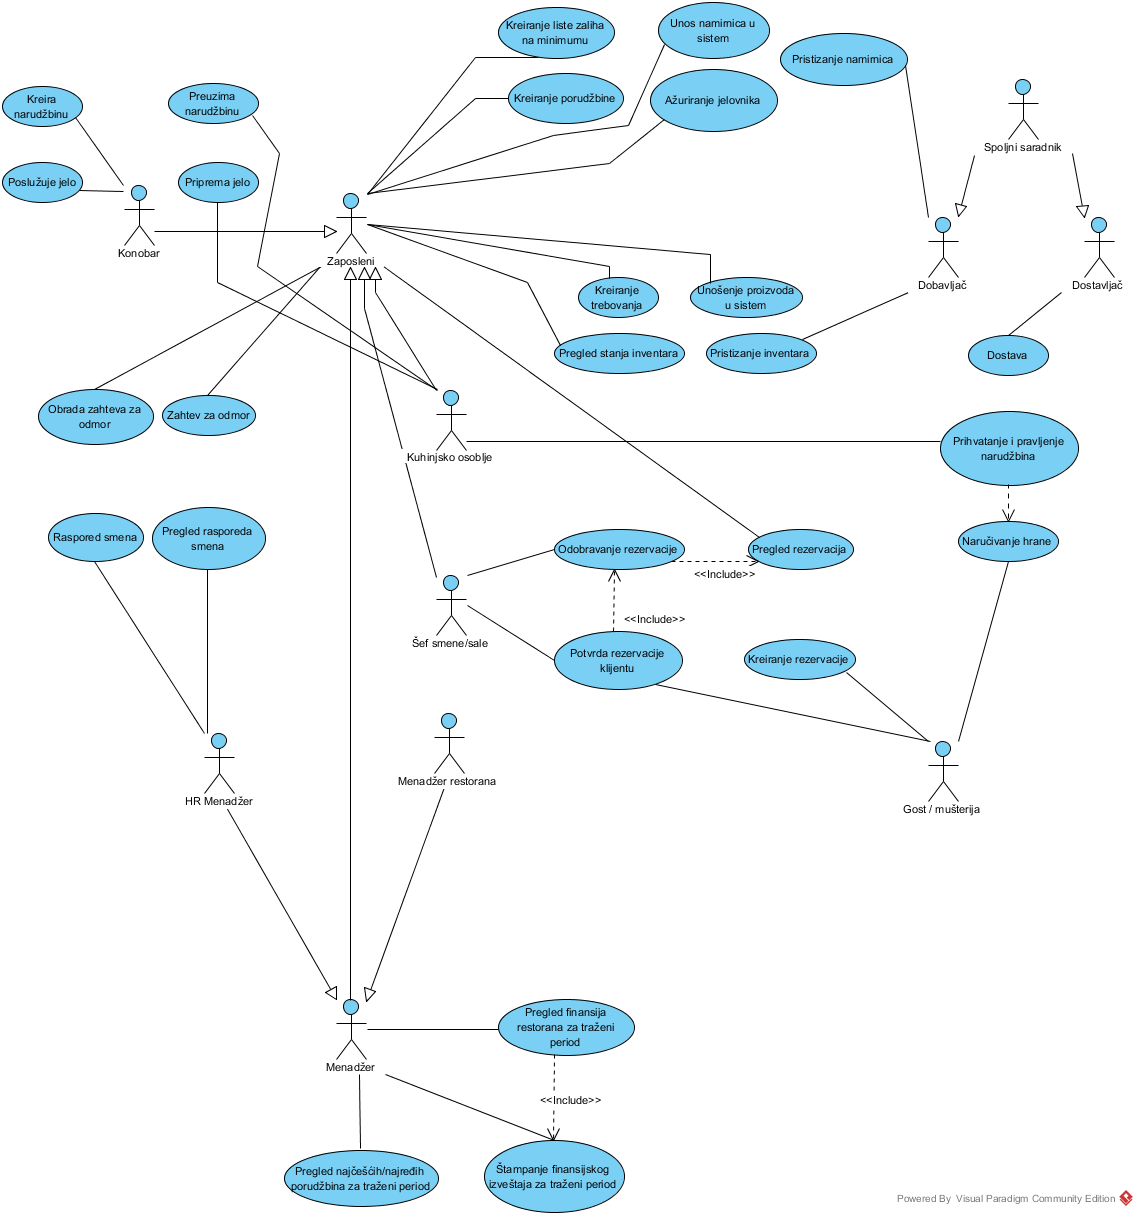
\includegraphics[width=\textwidth]{SU_0_grupni.png}
\pagebreak
\section{Slučajevi upotrebe}
Slučaj upotrebe (Use case, engl.) je specifikacija skupa akcija koje vrši sistem, koje proizvode vidljiv rezultat koji je, po pravilu, od vrednosti za jednog ili više učesnika u sistemu. Koristi se da precizira ponašanje sistema, bez otkrivanja njegove unutrašnje strukture.

%%%%%%%%%%%%%%%%%%%%%%%%%%%%%%%%%%%%%%%%%%%%%%%%%%%%%%%%%%%%%%%%%%%%%%%%%%%%

\subsection{Pregled stanja zaliha namirnica}
Pregled stanja zaliha namirnica je slučaj upotrebe u kojem se formalizuje način na koji ugostiteljski objekat planira nabavku namirnica, nabavlja, a potom ih dodaje na stanje. U tom procesu učestvuju menadžer nabavke (zaposleni) i dobavljač. 

\begin{itemize}
\item Zaposleni kreira spisak namirnica čija je trenutna količina ispod propisane minimalne. Na osnovu tog spiska, kreira porudžbinu. Kasnije, nakon isporuke porudžbine, unosi u bazu pristiglu robu.
\item Dobavljač isporučuje ugostiteljskom objektu namirnice u traženoj količini.
\end{itemize}
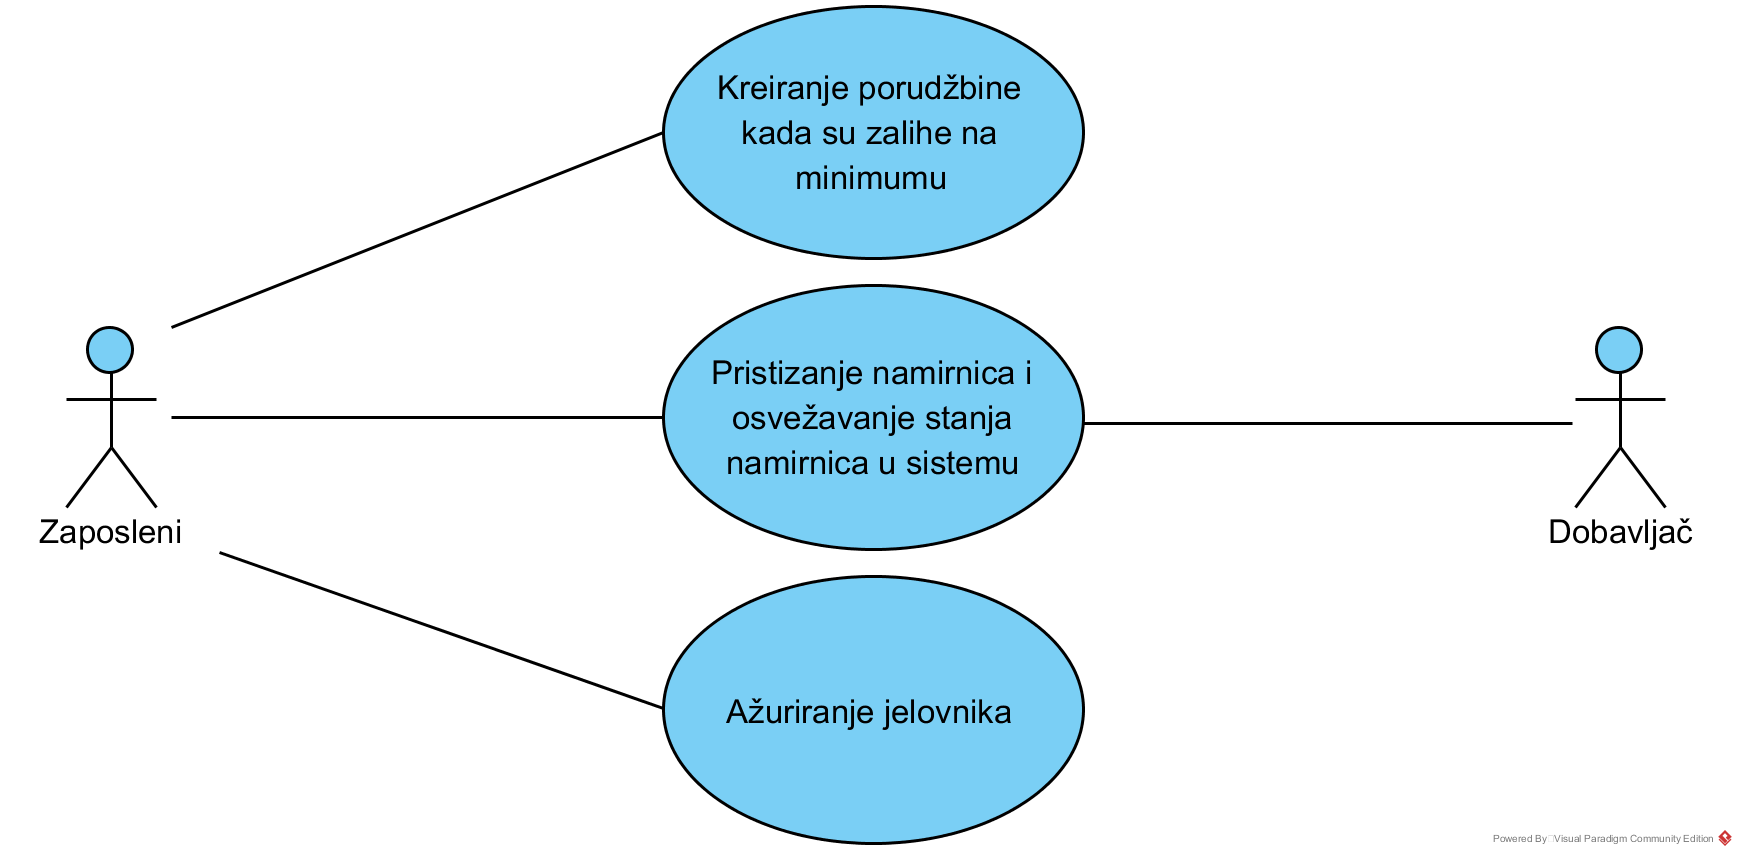
\includegraphics[width=\textwidth]{SU_1_zalihe.png}

\subsubsection{Kreiranje porudžbine kada su zalihe na minimumu}
Informacioni sistem omogućava lako kreiranje narudžbine za one namirnice čija dostupna količina je ispod definisanog minimuma neophodnog za pravilno funkcionisanje objekta.\\\\
\textbf{Akter:} Zaposleni\\
\textbf{Ulaz:} Lista namirnica čije su zalihe na minimumu.\\
\textbf{Izlaz:} Kreiran je i poručen spisak namirnica čije su zalihe na minimumu.\\
\textbf{Preduslovi:} Zaposleni se uspešno prijavio na glavni sistem gde se nalaze informacije o namirnicama.\\
\textbf{Postuslov:} Uspešno su poručene namirnice čija je količina manja od poželjne.\\
\textbf{Glavni tok:} 
\begin{enumerate}
	\item Zaposleni zahteva od sistema spisak namirnica za koje važi da je trenutna količina manja od minimalne propisane.
	\item Sistem generiše listu namirnica koje zadovoljavaju prethodno navedeni uslov.
	\item Zaposleni za svaku namirnicu procenjuje količinu za nabavku. 
	\item Zaposleni na spisak može dodati i namirnice kojih nema i nikada ih nije bilo u sistemu. 
	\item Zaposleni kreira porudžbinu.
\end{enumerate}
\textbf{Alternativni tokovi:} \\
\begin{itemize}
\item[1.1] Sistem ne može da generiše izveštaj ukoliko ne postoji proizvod sa minimalnom količinom, zaposleni prekida rad.
\item[2.1] Sistem nema spisak namirnica na minimalnim zalihama, tačnije spisak je prazan, procena se ne vrši, zaposleni završava rad.
\end{itemize}

\subsubsection{Pristizanje namirnica i osvežavanje stanja namirnica u sistemu}
Nove namirnice koje su isporučene restoranu, neophodno je uneti u informacioni sistem, da bi ostale komponente sistema bile svesne njihovog postojanja.\\\\
\textbf{Akter:} Dobavljač, zaposleni\\
\textbf{Ulaz:} Spisak namirnica koje je dobavljač isporučio.\\
\textbf{Izlaz:} Ažurirana je lista namirnica.\\
\textbf{Preduslovi:} Dobavljač je dostavio poručene namirnice. Zaposleni se uspešno prijavio na sistem. \\
\textbf{Postuslov:} Namirnice su isporučene kupcu i kreirana je lista dostavljenih proizvoda (Ažurirane su količine namirnica i eventualno su unete nove namirnice).\\
\textbf{Glavni tok:} 
\begin{enumerate}
	\item Dobavljač je primio porudžbinu.
	\item Dobavljač procenjuje da li je njegova firma u mogućnosti da odgovori na zahteve ugostiteljskog objekta.
	\item Dobavljač odlučuje za svaku namirnicu da li će isporučiti u smanjenoj ili traženoj količini.
	\item Dobavljač isporučuje robu ugostiteljskom objektu.
	\item Dobavljač pri isporuci dostavlja listu namirnica koje su isporučene.
    \item Zaposleni preuzima i potvrđuje listu isporučenih namirnica.
	\item Zaposleni za svaki od proizvoda sa liste ažurira proizvod u sistemu tako što dodaje pristiglu količinu.
	\item Zaposleni kreira novi proizvod ukoliko isti ne postoji u sistemu
	\item Zaposleni ažurira novokreiranu namirnicu pristiglom količinom i eventualno definiše minimalnu količinu. 
\end{enumerate}
\textbf{Alternativni tokovi:} 
\begin{itemize}
\item[2.1.] Dobavljač otkazuje porudžbinu zbog manjka raspoloživih namirnica, u 4. koraku lista dostavljenih namirnica je prazna.
\item[2.2.] Zaposleni kontaktira drugog dobavljača u cilju nabavke namirnica.
\end{itemize}

\subsubsection{Ažuriranje jelovnika}
Nakon svake nabavke, ili periodično, potrebno je izvršiti ažuriranje jelovnika, tako da se gostima nude ona i samo ona jela koje je moguće pripremiti na osnovu stanja zaliha namirnica u restoranu.\\\\
\textbf{Akter:} Zaposleni\\
\textbf{Ulaz:} Spisak namirnica u restoranu i spisak jela sa neophodnim namirnicama za njihovu pripremu.\\
\textbf{Izlaz:} Kreiran je jelovnik.\\
\textbf{Preduslovi:} Zaposleni se uspešno prijavio na sistem. Spisak jela i sastojaka od kojih se pripremaju nije prazan.\\
\textbf{Postuslov:} Jelovnik je kreiran. Gosti i zaposleni ga mogu videti.\\
\textbf{Glavni tok:} 
\begin{enumerate}
	\item Zaposleni zahteva od sistema ažuriranje jelovnika.
	\item Sistem na njegov zahtev kreira novi jelovnik tako što iz liste jela izbacuje ona za čiju pripremu nedostaje makar jedan sastojak.
	\item Sistem postavlja kreirani jelovnik za aktuelni jelovnik ugostiteljskog objekta.
\end{enumerate}
\textbf{Alternativni tokovi:}
\begin{itemize}
\item [1.1] Sistem nema podatke koji povezuju jela i namirnice te ne može generisati novi jelovnik; sistem ne ažurira ni aktuelni jelovnik. Zaposleni prekida sa radom.
\end{itemize}

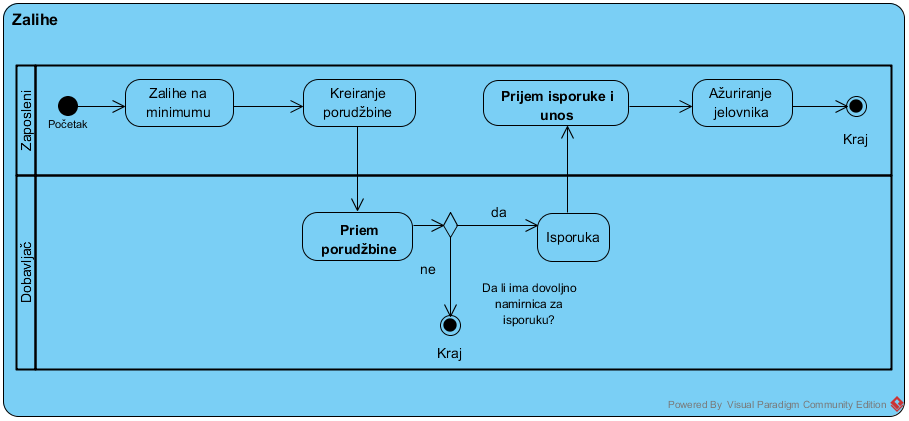
\includegraphics[width=\textwidth]{SU_1_zalihe_activity.png}

%%%%%%%%%%%%%%%%%%%%%%%%%%%%%%%%%%%%%%%%%%%%%%%%%%%%%%%%%%%%%%%%%%%%%%%%%%%%

\subsection{Pregled inventara}
Pregled inventara je slučaj upotrebe u kome se formalizuje način na koji ugostiteljski objekat planira nabavku inventara, nabavlja i ima uvid o stanju istog. U tom procesu učestvuju zaposleni i dobavljač. 

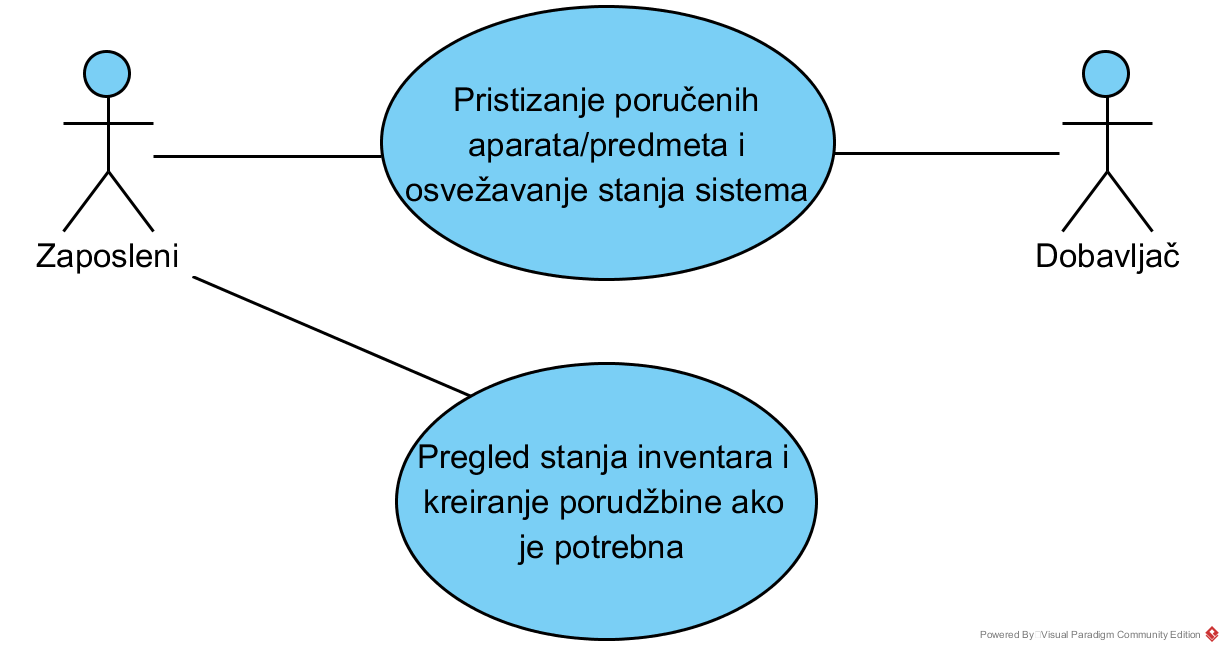
\includegraphics[width=\textwidth]{SU_2_pregled_inventara.png}
\subsubsection{Pregled stanja inventara i kreiranje porudžbine ako je potrebna}
Trenutno stanje inventara se pregleda, i porudžbina za nabavku artikala koji nedostaju se kreira po potrebi, radi normalnog kontinualnog funkcionisanja restorana.\\\\
\textbf{Akter:} Zaposleni\\
\textbf{Ulaz:} Nema\\
\textbf{Izlaz:} Lista predmeta koji su poručeni jer su zalihe ispod minimalnih definisanih za poslovanje ugostiteljskog objekta\\
\begin{enumerate}
	\item Spisak predmeta koji spadaju u inventar ugostiteljskog objekta i njihove zalihe su usled kvara ili nestanka ispod minimalnih definisanih količina.
	\item Lista svih predmeta i njihova trenutna količina.
\end{enumerate} 
\textbf{Preduslovi:} Zaposleni je uspešno ulogovan i ima uvid u spisak predmeta čija je količina manja od poželjne.\\
\textbf{Postuslov:} Uspešno je kreiran i poručen spisak predmeta. Ukoliko neki predmet zahteva popravku, lista sadrži tu informaciju.\\
\textbf{Glavni tok:} 
\begin{enumerate}
	\item Zaposleni zahteva od sistema spisak predmeta za koje važi da je trenutna količina manja od minimalne propisane ili je neki od aparata u kvaru.
	\item Sistem kreira listu predmeta koji ispunjavaju prethodni zahtev.
    \item Zaposleni uzima listu predmeta koje bi trebalo nabaviti.
	\item Zaposleni procenjuje količinu za nabavku. 
	\item Zaposleni proverava da li postoje predmeti koje želi da uvrsti u inventar i doda ih u porudžbinu.
	\item Zaposleni kreira porudžbinu.
\end{enumerate}
\textbf{Alternativni tokovi:}
\begin{itemize}
\item [1.1] Sistem nema podatke o minimalnim količinama ni za jedan predmet u sistemu, pa ne kreira pregled stanja. Zaposleni završava rad.
\item [3.1] Zaposleni ne vrši procenu ukoliko je lista predmeta na minimalnim zalihama prazna i završava sa radom.
\end{itemize}

\subsubsection{Pristizanje poručenih aparata/predmeta, i osvežavanje stanja sistema}
Nakon isporuke potraživanih predmeta, informacioni sistem se obaveštava o njihovom postojanju, tako da bi druge komponente informacionog sistema mogle biti osvežene novim podacima.\\\\
\textbf{Akter:} Dobavljač, zaposleni.\\
\textbf{Ulaz:} Spisak predmeta koje je dobavljač isporučio.\\
\textbf{Izlaz:} Predmeti su preuzeti i ažurirana je lista predmeta koji čine inventar.\\
\textbf{Preduslovi:} Dobavljač je dostavio poručene proizvode. Zaposleni se uspešno ulogovao na sistem.\\
\textbf{Postuslov:} Predmeti su isporučeni kupcu i ažurirane su količine proizvoda i eventualno uneti novi.\\
\textbf{Glavni tok:} 
\begin{enumerate}
	\item Dobavljač je dobio listu poručenih proizvoda.
	\item Dobavljač proverava za svaki proizvod da li je njegova firma u mogućnosti da isporuči tražene količine.
	\item Dobavljač po potrebi, smanjuje količine koje su poručene.
	\item Dobavljač isporučuje robu ugostiteljskom objektu.
	\item Dobavljač pri isporuci dostavljena je lista predmeta koji su isporučeni.  
    \item Zaposleni je dobio listu isporučenih proizvoda.
	\item Zaposleni za svaki od proizvoda sa liste ažurira proizvod u sistemu tako što dodaje pristiglu količinu.
	\item Ukoliko proizvod ne postoji u sistemu, radnik kreira proizvod sa njegovim karakteristikama.
	\item Zaposleni ažurira novokreirani proizvod pristiglom količinom i eventualno definiše minimalnu količinu. 
\end{enumerate}
\textbf{Alternativni tokovi:} 
\begin{itemize}
\item [2.1] Zbog manjka raspoloživih predmeta, dobavljač otkazuje porudžbinu.
\item [6.1] Porudžbina je otkazana, lista je prazna. Zaposleni završava rad.
\end{itemize}

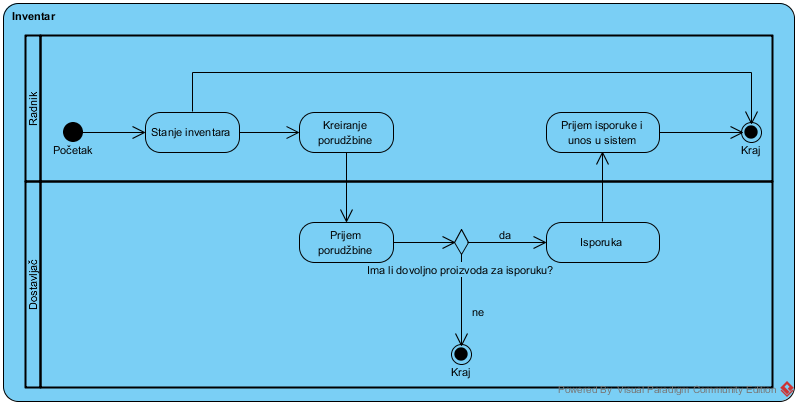
\includegraphics[width=\textwidth]{SU_2_pregled_inventara_activity.png}

%%%%%%%%%%%%%%%%%%%%%%%%%%%%%%%%%%%%%%%%%%%%%%%%%%%%%%%%%%%%%%%%%%%%%%%%%%%%

\subsection{Pregled finansijskog stanja}
Pregled finansijskog stanja je slučaj upotrebe u kojem menadžer restorana ima mogućnost pregleda prihoda i rashoda za dati vremenski period, koji se izračunavaju na osnovu naplaćenih usluga i troškova nabavke, održavanja, prihoda zaposlenih, itd.
\\
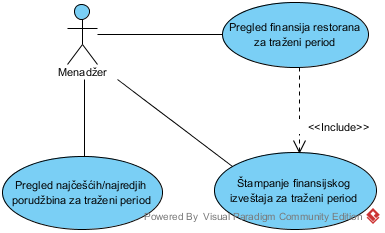
\includegraphics[width=\linewidth]{SU_3_pregled_finansija.png}

\subsubsection{Pregled finansijskog izveštaja za traženi period}
Finansijsko stanje restorana, koje uključuje prihode i rashode registrovane kroz informacioni sistem, pregleda se za traženi period i po potrebi štampa.\\\\
\textbf{Akter:} Menadžer\\
\textbf{Ulaz:} Datum početka perioda od interesa, datum kraja perioda od interesa, način štampanja.\\
\textbf{Izlaz:} Tabelarni prikaz prihoda i rashoda za traženi period i .pdf verzija finansijskog izveštaja.\\
\textbf{Preduslovi:} Menadžer se uspešno ulogovao na sistem i  ima pravo pristupa stranici za pregled finansija.\\
\textbf{Postuslov:} Odštampan finansijski izveštaj ima identične podatke kao i prikazani.\\
\textbf{Glavni tok:}
\begin{enumerate}
\item Menadžer vrši odabir početnog i krajnjeg dana perioda od interesa.
\item Menadžer dobija spisak prihoda i rashoda u datom vremenskom periodu.
\item Sistem prikazuje dijalog za štampu kreiranog izveštaja za navedeni period.
\end{enumerate}
\textbf{Alternativni tokovi:}\\
\begin{itemize}
\item [1.1.] Uneti datumi nisu validni, sistem prosleđuje poruku za ponovno unošnje datuma, nakon čega nastavlja ka koraku 2.
\item [2.1.] Za unete datume, restoran nije imao nijedan poslovni dan, sistem prikazuje adekvatnu poruku na ekranu i menadžer se preusmerava nazad na korak 1.
\item [2.2.] Korisnik ne želi da štampa izveštaj, već samo da ga pregleda.
\item [3.1.] Nijedan štampač nije povezan na sistem, prikazuje se poruka o grešci.
\end{itemize}
       
\subsubsection{Pregled najčešćih/najređih porudžbina za traženi period.}
Za traženi period, moguće je izvršiti pregled najčešćih/najređih porudžbina, radi upravljanja razvojem ugostiteljskog objekta, u smislu praćenja želja klijenata.\\\\
\textbf{Akter:} Menadžer\\
\textbf{Ulaz:} Datum početka perioda od interesa, datum kraja perioda od interesa.\\
\textbf{Izlaz:} Lista stavki sa menija koje su najčešće/najređe naručivane u traženom periodu.\\
\textbf{Preduslovi:} Menadžer se uspešno ulogovao na sistem i ima pravo pristupa stranici za pregled finansija.\\
\textbf{Postuslov:} Nema.\\
\textbf{Glavni tok:}
\begin{enumerate}
\item Menadžer vrši odabir početnog i krajnjeg dana perioda od interesa
\item Menadžer dobija spisak najčešće i najređe naručivanih stavki sa menija.
\end{enumerate}
\textbf{Alternativni tokovi:}\\
\begin{itemize}
\item [2.1.] Uneti datumi nisu validni, sistem prosleđuje poruku za ponovno unošenje datuma, nakon čega nastavlja ka koraku 2.
\item [3.1.] Za unete datume, restoran nije imao nijedan poslovni dan, prikazuje se adekvatna poruka na ekranu i korisnik se preusmerava nazad na korak 1.
\end{itemize}

%%%%%%%%%%%%%%%%%%%%%%%%%%%%%%%%%%%%%%%%%%%%%%%%%%%%%%%%%%%%%%%%%%%%%%%%%%%%

\subsection{Upravljanje ljudskim resursima}
Upravljanje ljudskim resursima je slučaj upotrebe u kojem se definišu rasporedi smena i godišnjih odmora. U planiranju učestvuju radnik i menadžer.

\begin{itemize}
\item Zaposleni svoje želje za godišnjim odmorom predaje na odobravanje menadžeru koji te želje prikuplja, obrađuje, planira i na kraju daje pozitivan ili negativan odgovor.
\item Raspored smena pravi menažer, koji su potom dostupni na pregled zaposlenima.
\end{itemize}
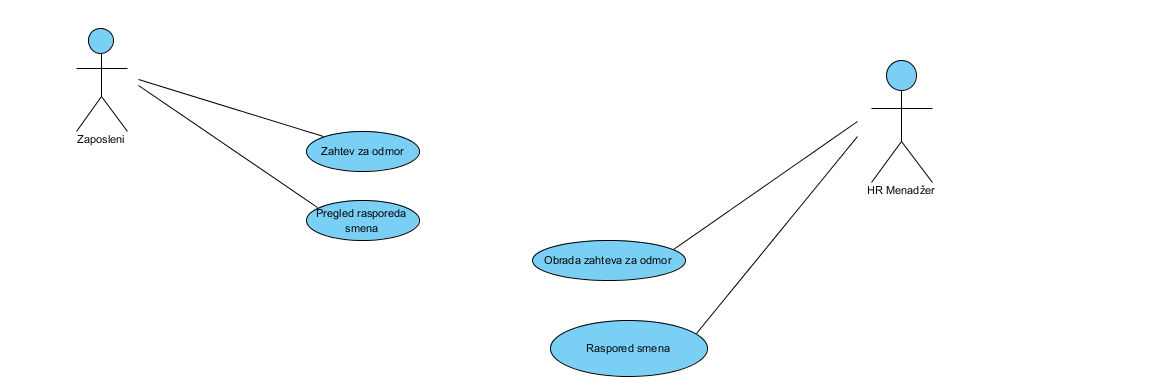
\includegraphics[width=\textwidth, height=100mm, keepaspectratio]{SU_4_hr.png}

\subsubsection{Pravljenje zahteva za odmor}
Da bi zaposleni ostvario svoje zagarantovano pravo na godišnji odmor, a i da bi organizacija rada bila moguća, mora pravovremeno podneti zahtev za godišnji odmor kroz informacioni sistem.\\\\
\textbf{Akter:} Zaposleni\\
\textbf{Ulaz:} Nema\\
\textbf{Izlaz:} Definisan zahtev za odmor\\
\textbf{Preduslovi:} Zaposleni se uspešno prijavio na sistem\\
\textbf{Postuslov:} Uspešno poslat zahtev za odmor\\
\textbf{Glavni tok:}
\begin{enumerate}
\item Zaposleni bira segment datuma za odmor.
\item Zaposleni potvrđuje izbor datuma i broj slobodnih dana za koji će biti umanjen njegov broj slobodnih dana.
\item Zahtev za odmor se evidentira u sistemu i prosleđuje na odobravanje menadžeru.
\end{enumerate}
\textbf{Alternativni tokovi:} \\
\begin{itemize}
\item [1.1.1] Uneti datumi nisu validni, sistem prosleđuje poruku za ponovno unošnje datuma, nakon čega nastavlja ka koraku 2.
\item [1.2.1] Zaposleni nema dovoljno slobodnih dana da bi poslao zahtev za odmor sa unetim datumima. Ponavlja se prvi korak.
\end{itemize}

\subsubsection{Obrada zahteva za odmor}
Pristigli zahtevi za ostvarivanje prava na godišnji odmor se obrađuju, i prihvataju ili odbijaju na osnovu stanja ostalih činilaca u restoranu za navedeni period.\\
\textbf{Akter:} Menadžer, zaposleni\
\textbf{Ulaz:} Spiskovi zahteva za odmor\\
\textbf{Izlaz:} Definisani odgovori na zahteve\\
\textbf{Preduslovi:} Menadžer se uspešno ulogovao na sistem i spiskovi zahteva su uspešno stigli do njega\\
\textbf{Postuslov:} Odgovori su definisani\\
\textbf{Glavni tok:}
\begin{enumerate}
\item Menadžer je obavešten da se pojavio novi zahtev za odmor (putem mejla).
\item Menadžer se loguje u sistem za evaluaciju odmora.
\item Za svakog zaposlenog sa spiska, menadžer posebno gleda da li je moguće organizovati funkcionisanje restorana u datom periodu bez dotičnog radnika.
\item Na osnovu procena stanja menadžer donosi odluku za svakog zaposlenog pojedinačno.
\item Za svakog zaposlenog pojedinačno, menadžer potvrđuje odgovor koji se dalje prosleđuje sistemu.
\item Zaposleni dobija informaciju da li je njegov zahtev za odmor odobren ili ne.
\end{enumerate}
\textbf{Alternativni tokovi:}\\
\begin{itemize}
\item[2.2.1.] Ukoliko su navedeni zahtevi za slobodnim danima definisani zakonom(slava, selidba, smrtni slučaj, rođenje deteta,..) dani menadžer ih odobrava bez dodatnih procena i prelazi na korak 3.
\end{itemize}

\subsubsection{Pravljenje rasporeda smena}
Radi normalnog funkcionisanja restorana, mora postojati jasan raspored smena zaposlenih, bez nepotrebnih preklapanja i sa dovoljnim brojem zaposlenih za svaki segment rada. To se postiže kreiranjem digitalnog rasporeda smena u informacionom sistemu, uz konsultovanje dostupnih informacija o potrebama procesa rada i raspoloživosti zaposlenih u datom periodu.\\\\
\textbf{Akter:} Menadžer\\
\textbf{Ulaz:} Nema\\
\textbf{Izlaz:} Novi raspored smena za određeni period je sačuvan u sistemu.\\
\textbf{Preduslovi:} Menadžer se uspešno ulogovao u sistem i postoje informacije o planu rada restorana za dati period kao i spisak godišnjih odmora.\\
\textbf{Postuslov:} Sastavljen je novi raspored smena za određeni period i sistem je ažuriran novim informacijama. Sistem obaveštava radnike o promenama.\\
\textbf{Glavni tok:} 
\begin{enumerate}
\item Menadžer definiše period za koji želi da napravi raspored smena.
\item Menadžer proverava plan rada restorana u datom periodu.
\item Menadžer proverava definisane godišnje odmore u datom periodu.
\item Na osnovu informacija dobijenih iz koraka 2 i 3 menadžer pravi raspored smena.
\item Menadžer ažurira sistem koji obaveštava radnike o definisanom rasporedu.
\end{enumerate}
\textbf{Alternativni tokovi:} \\
\begin{itemize}
\item [1.1.] Za dati period je već definisan raspored smena. Menadžer prelazi na korak 2 da bi menjao postojeći raspored.
\end{itemize}

\subsubsection{Pregled rasporeda smena}
Definisan raspored smena je moguće pregledati kroz informacioni sistem iz perspektive zaposlenog, za dati period od interesa.\\\\
\textbf{Akter:} Zaposleni\\
\textbf{Ulaz:} Nema\\
\textbf{Izlaz:} Raspored smena za zaposlenog\\
\textbf{Preduslovi:} Zaposleni se uspešno ulogovao u sistem\\
\textbf{Postuslov:} Uspešan pregled smena\\
\textbf{Glavni tok:}
\begin{enumerate}
\item Zaposleni unosi datum za koji želi da vidi svoj raspored smena.
\item Zaposleni ima na pregled raspored smena.
\end{enumerate}
\textbf{Alternativni tokovi:}\\
\begin{itemize}
\item [1.1.] Uneti datumi nisu validni, sistem prosleđuje poruku za ponovno unošnje datuma, nakon čega nastavlja ka koraku 2.
\item[2.1.] Još nije definisan raspored smena za izabrani datum. Zaposleni se može vratiti na 2. korak , ili izlogovati sa sistema.
\end{itemize}

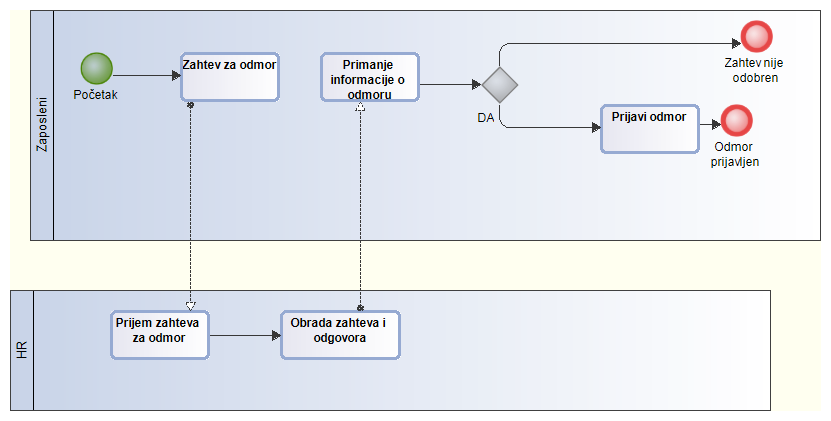
\includegraphics[width=\textwidth]{SU_4_Odmor.png}\\

%%%%%%%%%%%%%%%%%%%%%%%%%%%%%%%%%%%%%%%%%%%%%%%%%%%%%%%%%%%%%%%%%%%%%%%%%%%%

\subsection{Prihvatanje rezervacija gostiju}
\textbf{Prihvatanje rezervacija gostiju} je slučaj upotrebe u kojem se vrši prihvatanje i obrada digitalnih rezervacija mesta u restoranu. U tom procesu učestvuju potencijalni gost restorana, šef smene/sale restorana, kao i ostali zaposleni.\\

\begin{itemize}
\item Gost restorana posećuje stranicu za digitalne rezervacije i unosi sve potrebne podatke za rezervaciju
\item Šef smene ili sale odobrava rezervaciju na osnovu pregleda prethodno unetih rezervacija i potvrdjuje(ili odbija) rezervaciju potencijalnom gostu.
\end{itemize}
\vspace{1cm}
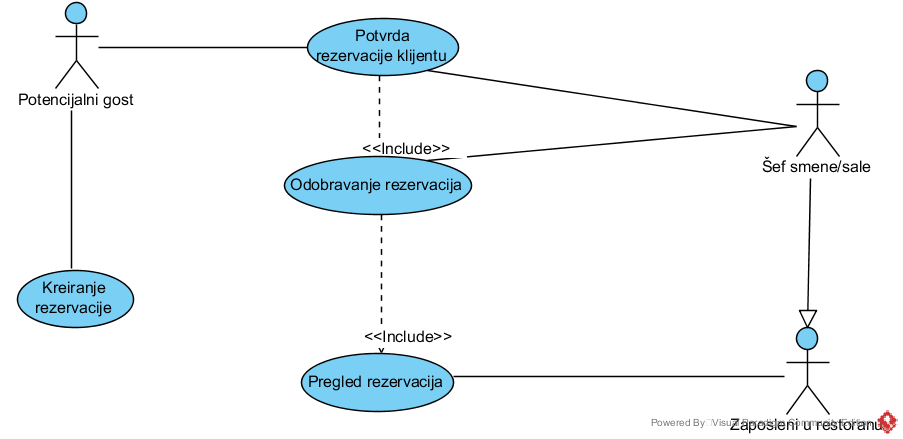
\includegraphics[width=\textwidth]{SU_5_prihvatanje_rezervacija.png}

\subsubsection{Kreiranje rezervacije}
Potencijalni gost restorana kreira rezervaciju posredstvom informacionog sistema.\\\\
\textbf{Akter:} Gost\\
\textbf{Ulaz:} Kontakt podaci gosta (ime, prezime, kontakt telefon ili e-mail adresa), datum rezervacije, broj gostiju, specijalne napomene\\
\textbf{Izlaz:} Redni broj zahteva za rezervaciju.\\
\textbf{Preduslovi:} Nema.\\
\textbf{Postuslov:} Uspešno je kreiran zahtev za rezervaciju.\\
\textbf{Glavni tok:}
\begin{enumerate}
\item Gost vrši navigaciju na stranu za rezervaciju
\item Gost unosi zahtevane podatke
\item Gost šalje restoranu zahtev za rezervaciju
\item Gost dobija potvrdu da je zahtev za rezervaciju dostavljen restoranu na obradu.\\
\end{enumerate}
\textbf{Alternativni tokovi:}\\
\begin{itemize}
\item [4.1.] Sistem ne prosleđuje potvrda o poslatom zahtevu u roku od 2 minuta.
\item [4.1.1.] Sistem prikazuje poruku sa izvinjenjem i kontakt telefonom kojim se rezervacija može izvršiti "offline".
\end{itemize}

\subsubsection{Pregled rezervacija}
Rezervacije koje su registrovane u informacionom sistemu mogu biti pregledane od strane zaposlenih u restoranu.\\\\
\textbf{Akter:} Zaposleni\\
\textbf{Ulaz:} Datum i/ili broj stola za koji se pregleda spisak rezervacija.\\
\textbf{Izlaz:} Spisak registrovanih rezervacija koje odgovaraju kriterijumu pretrage.\\
\textbf{Preduslovi:} Zaposleni se uspešno prijavio na sistem.\\
\textbf{Postuslov:} Nema.\\
\textbf{Glavni tok:}
\begin{enumerate}
\item Zaposleni unosi ulazne parametre
\item Zaposleni dobija tabelarni prikaz registrovanih rezervacija koje zadovoljavaju kriterijume pretrage.\\
\end{enumerate}
\textbf{Alternativni tokovi:} \ \\

\subsubsection{Odobravanje rezervacija}
Svaka rezervacija koja je pristigla u informacioni sistem se odobrava od strane ovlašćenog osoblja, na osnovu trenutnog stanja restorana (slobodna mesta, materijal za rad).\\\\
\textbf{Akter:} Šef smene/sale\\
\textbf{Ulaz:} Podaci iz pristiglog zahteva za rezervaciju, informacije o već registrovanim rezervacijama i raspoloživom broju i strukturi mesta.\\
\textbf{Izlaz:} Rezervacija odobrena ili odbijena i redni broj rezervacije.\\
\textbf{Preduslovi:} Šef se uspešno prijavio na sistem i ima pravo da pristupi odobravanju rezervacija.\\
\textbf{Postuslov:} Informacije o odobrenim rezervacijama su sačuvane u sistemu.\\
\textbf{Glavni tok:}
\begin{enumerate}
\item Šef pregleda spisak dospelih zahteva za rezervaciju
\item Šef za svaki od zahteva vrši pregled rezervacija da bi utvrdio da li je rezervacija sa zadatim parametrima moguća
\item Šef odobrava ili odbija rezervaciju i svoju odluku registruje u sistemu.\\
\end{enumerate}
\textbf{Alternativni tokovi:}\\
\begin{itemize}
\item [1.1.] Spisak je prazan, šef završava sa radom.
\end{itemize}

\subsubsection{Uklanjanje registrovanih rezervacija}
Rezervacija se uklanja ukoliko za to postoji opravdan razlog.\\\\
\textbf{Akter:} Šef smene/sale\\
\textbf{Ulaz:} Redni broj rezervacija koju treba obrisati i razlog brisanja.\\
\textbf{Izlaz:} Nema.\\
\textbf{Preduslovi:}Šef se uspešno prijavio na sistem i ima pravo da pristupi meniju za uklanjanje registrovanih rezervacija. Postoji validan razlog za uklanjanje rezervacije koji je iskomuniciran sa gostom (sa čije god strane da je razlog potekao).\\
\textbf{Postuslov:} Rezervacija sa datim rednim brojem je uklonjena iz sistema i razlog uklanjanja je registrovan.\\
\textbf{Glavni tok:}
\begin{enumerate}
\item Šef unosi ulazne podatke
\item Šef uklanja rezervaciju iz sistema
\item Sistem prikazuje preostale rezervacije za isti datuma kao kod uklonjene rezervacije.\\
\end{enumerate}
\textbf{Alternativni tokovi:}\\
\begin{itemize}
\item [2.1.] Rezervacija sa datim rednim brojem ne postoji u sistemu. Sistem prikazuje grešku i prikazuje spisak poslednjih deset uklonjenih rezervacija, šef zaršava sa radom.
\end{itemize}

\subsubsection{Potvrda rezervacije gostu}
Gostu čija je rezervacija odobrena, potvrđuje se prijem i prihvatanje rezervacije na osnovu kontakt podataka prisutnih u informacionom sistemu. Ovaj korak je neophodan radi sprečavanja zloupotrebe digitalnog sistema za rezervaciju.\\\\
\textbf{Akter:} Šef smene/sale, gost.\\
\textbf{Ulaz:} Redni broj rezervacije i kontakt podaci gosta.\\
\textbf{Izlaz:} Rezervacija je potvrdjena ili ne.\\
\textbf{Preduslovi:} Šef se uspešno prijavio na sistem i ima pravo da pristupi meniju za potvrđivanje rezervacija.\\
\textbf{Postuslov:} Rezervacija je potvrđena.\\
\textbf{Glavni tok:}
\begin{enumerate}
\item Šef pregleda odabranu rezervaciju
\item Šef šalje potvrdu gostu automatski generisanom elektronskom poštom ili poziva gosta telefonom.\\
\end{enumerate}
\textbf{Alternativni tokovi:}\\
\begin{itemize}
\item [2.1.] Kontakt podaci nisu validni, šef rezervaciju se  registruje kao uklonjenu, sa razlogom "nevalidni kontakt podaci gosta".
\end{itemize}
  
%%%%%%%%%%%%%%%%%%%%%%%%%%%%%%%%%%%%%%%%%%%%%%%%%%%%%%%%%%%%%%%%%%%%%%%%%%%%

\subsection{Online naručivanje i dostava hrane i pića}
Online naručivanje i dostava hrane i pića je slučaj upotrebe gde mušterija definiše svoju narudžbinu, radnici je prave, a dostavljači isporučuju. U naručivaju učestvuju: mušterija, radnik i dostavljač.\\\\
\\
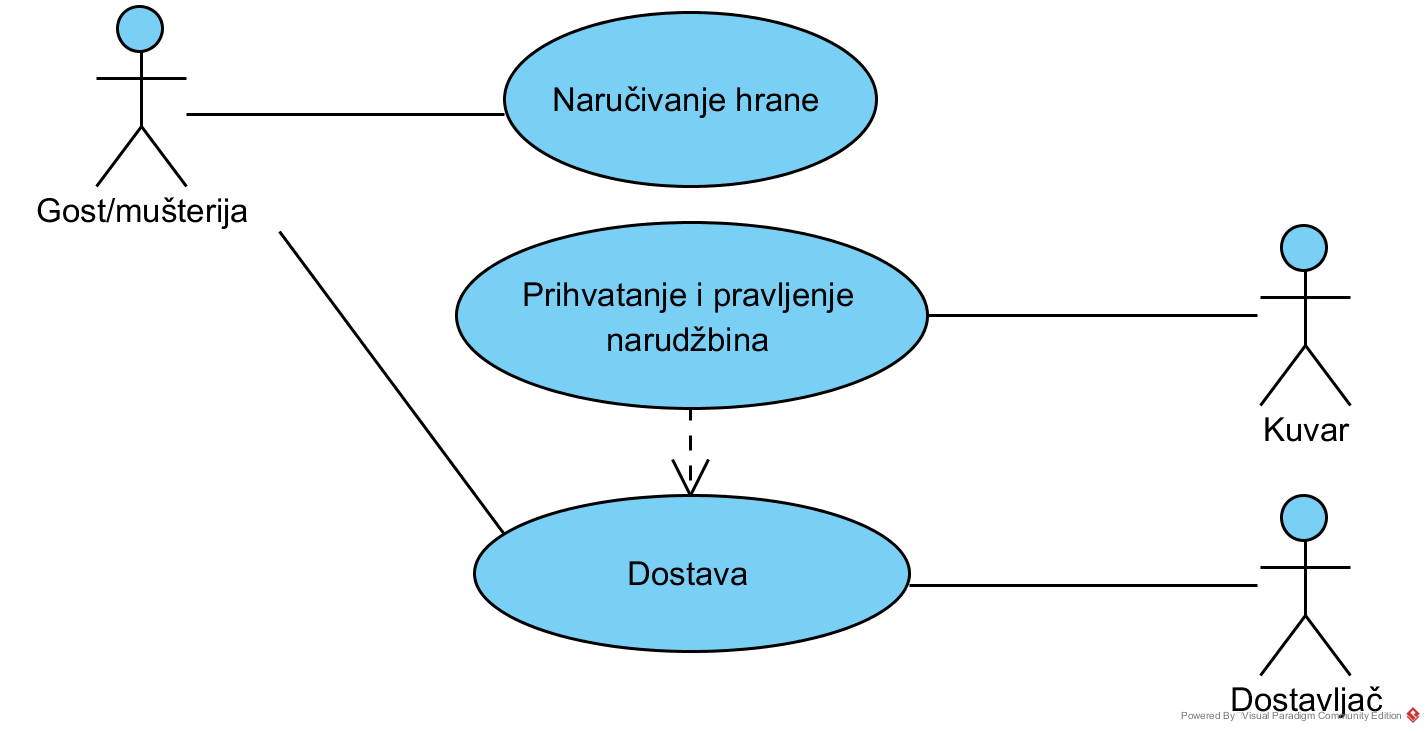
\includegraphics[width=\linewidth]{SU_6_dostava.png}

\subsubsection{Naručivanje hrane}
Mušterija vrši odabir hrane i pića i kreira narudžbinu.\\
\textbf{Akter:} Mušterija\\
\textbf{Ulaz:} Kontakt podaci mušterije (ime, prezime, kontakt telefon ili e-mail adresa), datum rezervacije, broj gostiju, specijalne napomene\\
\textbf{Izlaz:} Definisana narudžbina\\
\textbf{Preduslovi:} Restoran prima narudžbine\\
\textbf{Postuslov:} Uspešno napravljena narudžbina je poslata restoranu\\
\textbf{Glavni tok:}
\begin{enumerate}
\item Mušterija vrši odabir hrane i pića.
\item Mušerija potvrđuje narudžbinu.
\item Mušerija dobija potvrdu da je narudžbina dostavljena restoranu na obradu.\\
\end{enumerate}
\textbf{Alternativni tokovi:} \\
\begin{itemize}
\item [3.1.] Sistem ne prosleđuje potvrdu o poslatom zahtevu u roku od 2 minuta.
\item [3.1.1.] Sistem prikazuje poruku sa izvinjenjem i kontakt telefonom kojim se narudžbina može izvršiti "offline".
\item [3.1.1.] Nakon odabira akcije mušterija završava sa radom.
\end{itemize}


\subsubsection{Prihvatanje i pravljenje narudžbina}
Radnik pravi svaku pristiglu narudžbinu, zatim obaveštava dostavljača o mogućnosti dostave.\\
\textbf{Akter:} Radnik, dostavljač\\
\textbf{Ulaz:} Spisak narudžbina\\
\textbf{Izlaz:} Napravljene narudžbine\\
\textbf{Preduslovi:} Radnik se uspešno ulogovao na sistem i spiskovi narudžbina su uspešno stigli do njega\\
\textbf{Postuslov:}  Napravljene narudžbine su spremne za dostavu\\
\textbf{Glavni tok:}
\begin{enumerate}
\item Radnik uzima spiskove narudžbina.
\item Radnik za svaku narudžbinu iz spiska pravi porcije, po redosledu vremena naručivanja.
\item Po završetku pravljenja obroka, radnik obaveštava dostavljača da je porudžbina spremna za dostavu 
\end{enumerate}
\textbf{Alternativni tokovi:}\\
\begin{itemize}
\item [2.1.] Ukoliko  fale sastojci za neku od narudžbina, prelazi se na sledeću narudžbinu dok sastojci ne stignu.
\end{itemize}
       
\subsubsection{Dostava}
Napravljenu narudžbinu dostavljač odnosi na adresu navedenu u samom zahtevu.\\
\textbf{Akter:} Dostavljač, mušterija\\
\textbf{Ulaz:} Pripremljena narudžbina\\
\textbf{Izlaz:} Izvršena dostava\\
\textbf{Preduslovi:} Mušterija je ispravno definisala adresu\\
\textbf{Postuslov:}  Izvršena dostava je plaćena\\
\textbf{Glavni tok:}
\begin{enumerate}
\item Dostavljač odnosi porudžbina na adresu definisanu na narudžbini
\item Mušterija prihvata porudžbinu i proverava da li je sve u redu sa sadržajem
\item Mušterija plaća dostavu
\end{enumerate}
\textbf{Alternativni tokovi:}\\
\begin{itemize}
\item [2.1.]  Ukoliko nije sve u redu sa sadržajem, mušterija pravi novu narudžbnu i čeka novu dostavu, ili mušterija odustaje od narudžbine.
\item [2.1.1] Ukoliko je mušterija odustala, dostavljač vraća hranu u restoran.
\end{itemize}

%%%%%%%%%%%%%%%%%%%%%%%%%%%%%%%%%%%%%%%%%%%%%%%%%%%%%%%%%%%%%%%%%%%%%%%%%%%%

\subsection{Obrada porudžbine gosta}
Obrada porudžbine gosta je slučaj upotrebe u kojem gost biva uslužen od strane osoblja restorana uz razmenu informacija između gosta i kuhinje posredstvom informacionog sistema.

\subsubsection{Gost poručuje jelo}
Gost nakon pregledanja restoranskog menija poručuje jelo od konobara, koji narudžbinu prosledjuje do kuhinjskog osoblja posredstvom informacionog sistema.\\\\
\textbf{Akteri:} Gost, konobar, kuhinjsko osoblje\\
\textbf{Ulaz:} Jelovnik.\\
\textbf{Izlaz:} Osvežen globalni spisak porudžbina novom porudžbinom.\\
\textbf{Preduslov:} Gost je u restoranu.\\
\textbf{Postuslov:} Uspešno je napravljen skup porudžbina gosta i upisan u globalni spisak porudžbina.\\
\textbf{Glavni tok:}
\begin{enumerate}
\item Gost potražuje jelo sa menija
\item Konobar beleži narudžbinu 
\item Konobar dodaje porudžbinu na listu porudžbina.
\item Kuhinjsko osoblje prati promene na listi porudžbina, i u skladu sa time započinje pripremu jela \\
\end{enumerate}

\subsubsection{Konobar isporučuje jelo}
Konobar preuzima gotova jela iz kuhinje nakon signala dobijenog posredstvom informacionog sistema i završava proces usluživanja gosta.\\\\
\textbf{Akteri:} Gost, konobar, kuhinjsko osoblje\\
\textbf{Ulaz:} Gotovo jelo koje je konobar preuzeo iz kuhinje.\\
\textbf{Izlaz:} Posluženo jelo.\\
\textbf{Preduslov:} Pripremljena sva jela sa odabrane porudžbine.\\
\textbf{Postuslov:} Gostu je posluženo jelo.\\
\textbf{Glavni tok:}
\begin{enumerate}
\item Kuhinjsko osoblje nakon završetka pripreme svih jela sa porudžbine gosta osvežava status porudžbine u listi porudžbina
\item Konobar preuzima jela i uslužuje ih gostu \\
\end{enumerate}
\textbf{Alternativni tokovi:}
\begin{enumerate}
\item Nema svih sastojaka potrebnih za pripremu jela.
\item Kuhinjsko osoblje naručuje potrebne sastojke, ukoliko ne mogu da stignu u određenom vremenskom periodu, kontaktira se konobar da pita mušteriju za drugi odabir. 
\end{enumerate}

  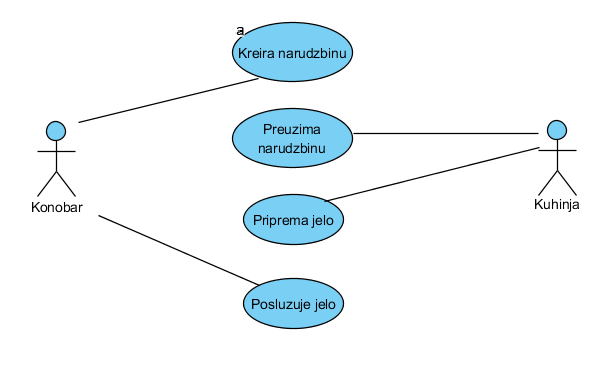
\includegraphics[width=\textwidth]{SU_7_konobar_kuhinja.png}
  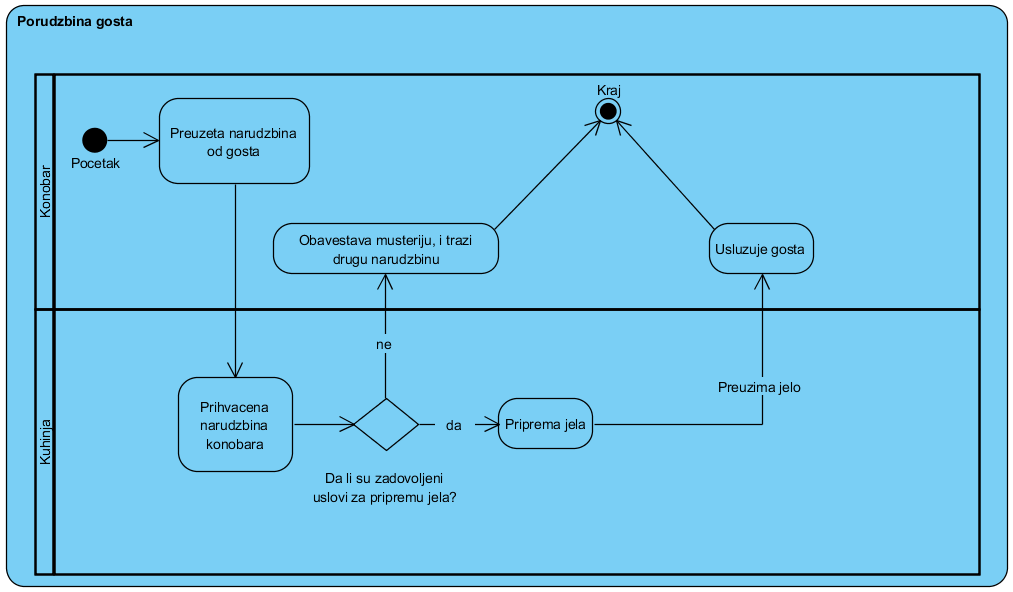
\includegraphics[width=\textwidth]{SU_7_porudzbina.png}
\pagebreak

%%%%%%%%%%%%%%%%%%%%%%%%%%%%%%%%%%%%%%%%%%%%%%%%%%%%%%%%%%%%%%%%%%%%%%%%%%%%

\section{Baza podataka}
\subsection{Pregled šeme baze podataka}
Na sledećoj slici može se videti šema baze podataka koja je deo implementacije informacionog sistema (\href{https://raw.githubusercontent.com/bozidarrr/NajmanjiProblem/master/FinalniDokument/NajmanjiProblem_BazaPodataka.png}{Slika visoke rezolucije}):\\
\vspace{1mm}
 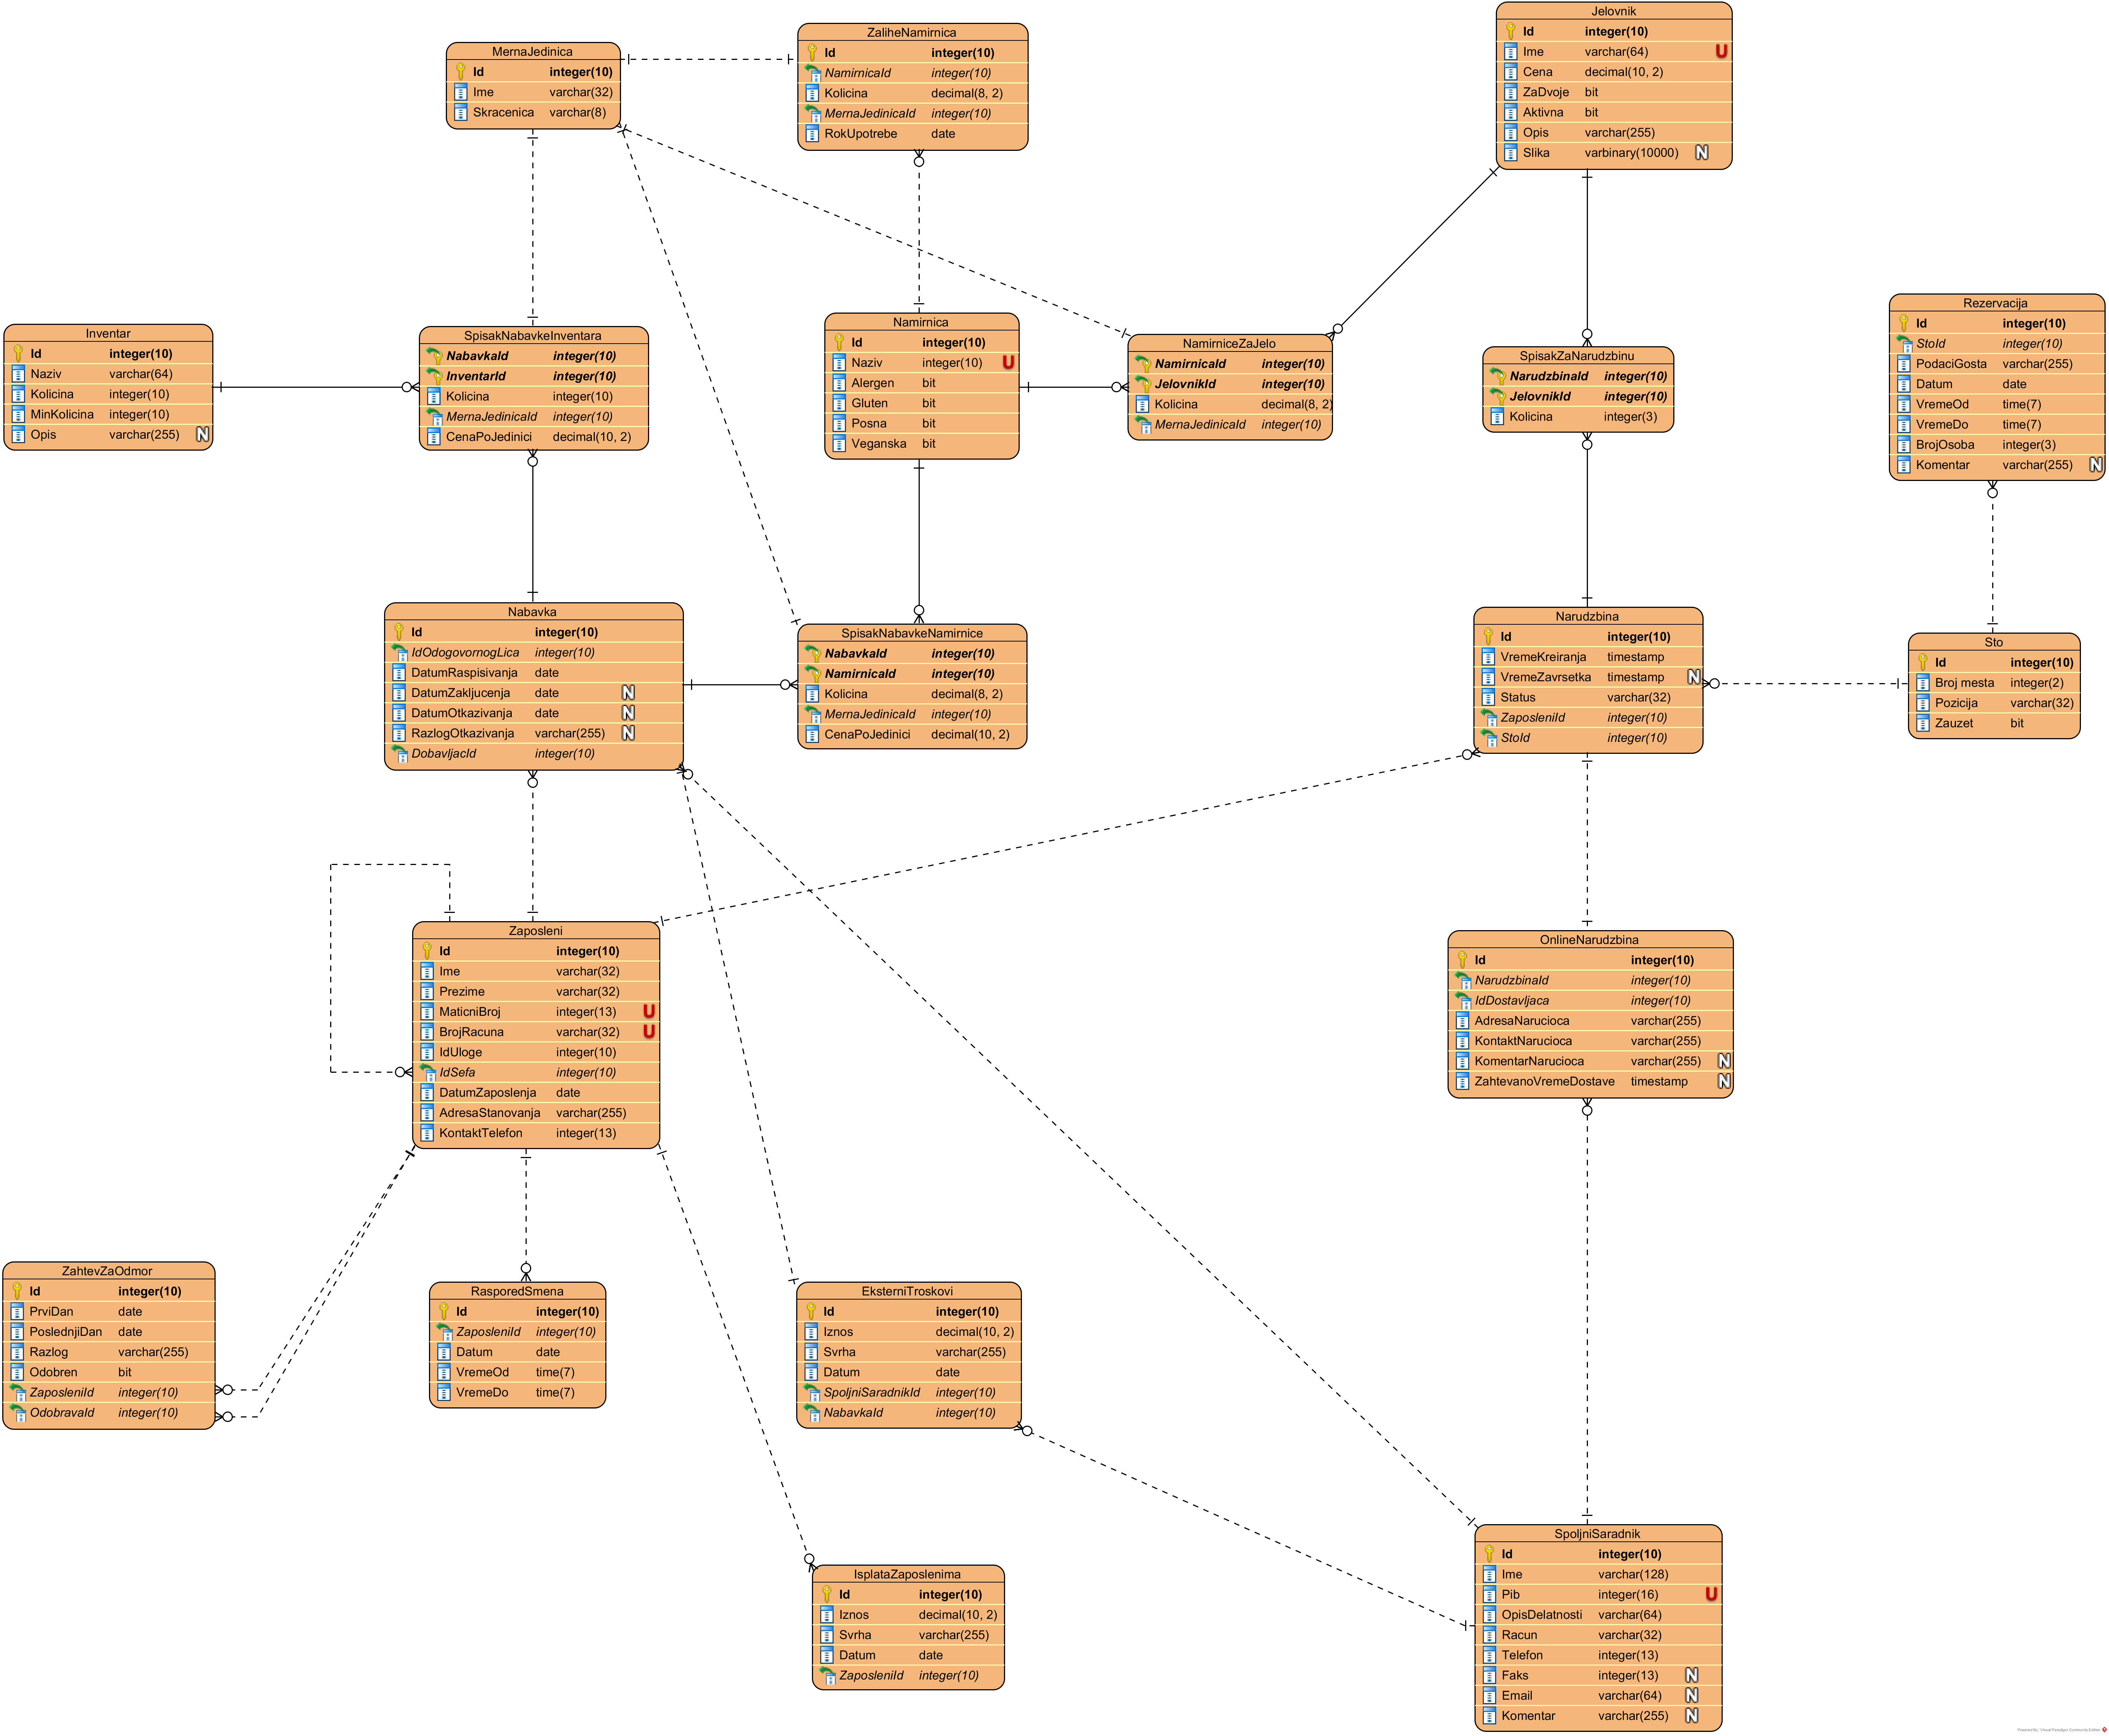
\includegraphics[width=\textwidth]{NajmanjiProblem_BazaPodataka.png}
 
\subsection{Opis operacija nad bazom prema slučajevima upotrebe}
\subsubsection{Kreiranje porudžbine kada su zalihe na minimumu}
\begin{itemize}
\item Pregled odgovarajućeg pogleda \emph{ZaliheNaIsteku}.
\item Dodavanje novog reda u \emph{Nabavka}.
\item Za svaku stavku koja se traži, dodaje se novi red u \emph{SpisakNabavkeInventara} sa predmetom i količinom.
\item Ako novi predmet nije postojao, dodaje se i novi red u \emph{Inventar}, gde je podrazumevana vrednost za \emph{Kolicina} 0, a \emph{MinKolicina} se postavlja ručno.
\end{itemize}

\subsubsection{Pristizanje namirnica i osvežavanje stanja namirnica u sistemu}
\begin{itemize}
\item Poziv odgovarajuće stored procedure koja upisuje datum zaključenja nabavke, ažuriranje tabele \emph{Zalihe} namirnica sa ručnim unošenjem roka upotrebe unetih artikala.
\item Unos novog reda u tabelu \emph{Namirnice} sa potrebnim podacima.
\end{itemize}

\subsubsection{Ažuriranje jelovnika}
\begin{itemize}
\item Vrši se automatski postavljanjem oznake omogućeno/onemogćeno od strane odgovarajućeg trigera nakon svakog uklanjanja namirnice sa stanja zaliha odnosno nakon unosa namirnica u sistem.
\end{itemize}

%%%%%%%%%%%%%%%%%%%%%%%%%%%%%%%%%%%%%%%%%%%%%%%%%%%%%%%%%%%%%%%%%%%

\subsubsection{Pristizanje poručenih aparata/predmeta i osvežavanje stanja sistema}
\begin{itemize}
\item Pregleda se spisak \emph{Nabavka x SpisakNabavkeInventara}, i poziva se stored procedura koja validira nabavku, unosi \emph{DatumPristizanja}, povećava količinu za svaku pogođenu stavku inventara 
\item Unošenje novog reda u tabelu \emph{Inventar}, sa količinom jednakom nuli kao podrazumevano. Mora postojati dokaz o nabavci, tako da veličina veca od nule za početnu vrednost ne bi trebalo da ima smisla
\end{itemize}

\textbf{Pregled stanja inventara i kreiranje porudžbine ako je potrebna} :
\begin{itemize}
\item Pregled tabele \emph{Inventar}. Zahteva se primarni indeks na id koloni zbog joinova i na naziv radi lake pretrage po nazivu (nonclustered).
\item Druga varijanta, pregled view-a \emph{InventarNaIzmaku} koji sadrži samo one stavke koje su jako blizu ili ispod granice \emph{MinKolicina} za funkcionisanje.
\item Kreiranje novog reda u tabeli \emph{Nabavka}.
\end{itemize}

%%%%%%%%%%%%%%%%%%%%%%%%%%%%%%%%%%%%%%%%%%%%%%%%%%%%%%%%%%%%%%%%%%%

\subsubsection{Pregled finansijskog izveštaja restorana za traženi period}
\begin{itemize}
\item  Podaci se dobijaju iz odgovarajućeg pogleda, koji objedinjuje podatke iz spiska odliva zbog nabavki (a preko \emph{SpiskaNabavkiNamirnica} i \emph{SpiskaNabavkeInventara} ), materijalnih troskova (\emph{IsplataZaposlenima} i \emph{EksterniTroskovi}) kao i priliva na osnovu podataka povezanih sa narudžbinama. 
\end{itemize}

\subsubsection{Pregled najčešćih/najređih narudžbina za traženi period}
\begin{itemize}
\item Podaci se dobijaju iz odgovarajućeg pogleda, na osnovu podataka iz tabele \emph{Narudžbina} i sa njom povezanih spiskova.
\end{itemize}

%%%%%%%%%%%%%%%%%%%%%%%%%%%%%%%%%%%%%%%%%%%%%%%%%%%%%%%%%%%%%%%%%%%

\subsubsection{Pravljenje zahteva za odmor}
\begin{itemize}
\item Vrši se insert novog reda u tabelu \emph{ZahtevZaOdmor} 
\end{itemize}

\subsubsection{Pregled rasporeda smena}
\begin{itemize}
\item Vrši se pregled tabele raspored smena, tako što se za vrednosti koje nisu pokrivene nijednim unosom smatra da niko nije raspoređen
\end{itemize}

\subsubsection{Obrada zahteva za odmor}
\begin{itemize}
\item U odgovarajućem zahtevu za odmor se menja flag odobren.
\item Aktivira se triger koji u rasporedu smena uklanja zaposlenog iz rasporeda u periodu kada je na odmoru.
\end{itemize}

\subsubsection{Pravljenje rasporeda smena}
\begin{itemize}
\item Za dati datum se unosi po jedan red za svakog zaposlenog, za svaki kontinualni segment rada. Odgovarajućom stored procedurom se može ponoviti raspored i za sledeći dan.
\end{itemize}

%%%%%%%%%%%%%%%%%%%%%%%%%%%%%%%%%%%%%%%%%%%%%%%%%%%%%%%%%%%%%%%%%%%

\subsubsection{Kreiranje rezervacija}
\begin{itemize}
\item  Dodaje se novi red u tabelu rezervacija ukoliko je to moguće zbog ograničenja 
\end{itemize}


\subsubsection{Pregled rezervacija}
\begin{itemize}
\item Vrši se pregled tabele za rezervacije 
\end{itemize}


\subsubsection{Odobravanje rezervacija}
\begin{itemize}
\item Dodeljuje se NOT NULL vrednost za StoId 
\end{itemize}

\subsubsection{Potvrda rezervacije}
\begin{itemize}
\item Menjaju se podaci ukoliko je potrebno. Ukoliko nema uspešne potvrde, rezervacija se briše iz sistema.
\end{itemize}

%%%%%%%%%%%%%%%%%%%%%%%%%%%%%%%%%%%%%%%%%%%%%%%%%%%%%%%%%%%%%%%%%%%

\subsubsection{Naručivanje hrane}
\begin{itemize}
\item Kreiranje online narudžbine unosi novi red u \emph{OnlineNarudzbina}. To dalje kreira narudžbinu kao i u prethodnom slučaju.
\end{itemize}

\subsubsection{Prihvatanje i pravljenje narudžbina}
\begin{itemize}
\item Isto kao za preuzimanje narudžbina, pošto je tabela \emph{Naruzdbina} ono sto kuhinja zapravo vidi
\end{itemize}


\subsubsection{Dostava}
\begin{itemize}
\item Menja se status narudzbine na odgovarajući kada dostavljač potvrdi dostavu
\end{itemize}

%%%%%%%%%%%%%%%%%%%%%%%%%%%%%%%%%%%%%%%%%%%%%%%%%%%%%%%%%%%%%%%%%%%

\subsubsection{Gost poručuje jelo}
\begin{itemize}
\item Unosi se novi red za svaki sto koji je zahvaćen narudžbinom i pravi se odgovarajući spisak za narudžbinu
\item Nakon što je priprema gotova, menja se status narudžbine na odgovarajući način
\end{itemize}

\subsubsection{Konobar isporučuje jelo}
\begin{itemize}
\item Menja se status narudžbine 
\item Menja status narudžbine i registruje njen završetak
\item Pri uklanjanju pribora sa stola, sto se markira kao slobodan
\end{itemize}

%%%%%%%%%%%%%%%%%%%%%%%%%%%%%%%%%%%%%%%%%%%%%%%%%%%%%%%%%%%%%%%%%%%%%%%%%%%%

\section{Predlog korisničkog interfejsa}

\subsection{Deo aplikacije namenjen za zaposlene}
\subsubsection{Prijavljivanje na sistem}
Na stranici za prijavljivanje na sistem korisnik treba da unese korisničko ime i lozinku.\\

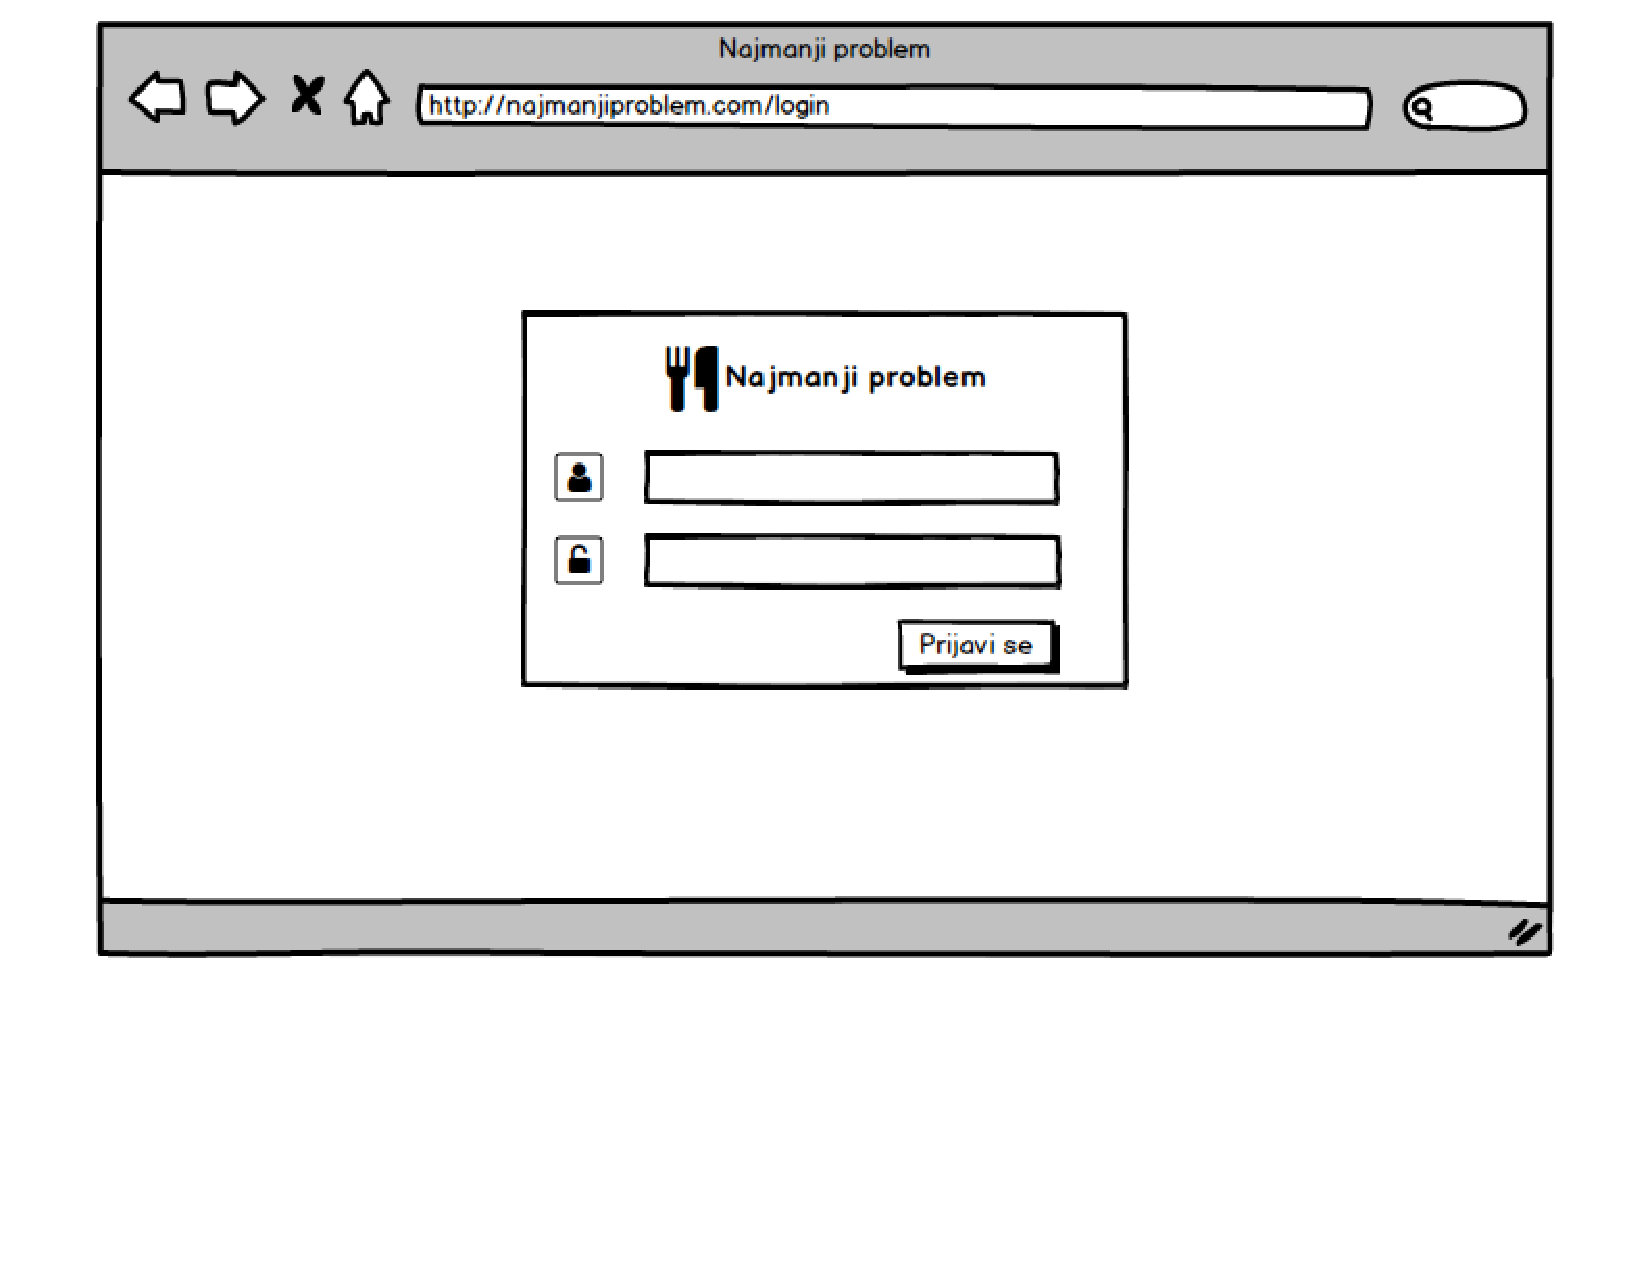
\includegraphics[
    page=1,
    width=\textwidth,
    height=\textheight,
    keepaspectratio]{0_PrijavljivanjeNaSistem.pdf}

\subsubsection{Pregled stanja zaliha namirnica}
Na panelu za \emph{Namirnice} korisnik može da generiše spisak namirnica potrebnih za nabavku i da ih odmah i naruči. Može da vrši preragu po namirnicama, a može i da kreira novu namirnicu. Na panelu \emph{Jelovnik} moguće akcije su ažuriranje postojećeg jelovnika, pretraga i kreiranje novog jelovnika.\\

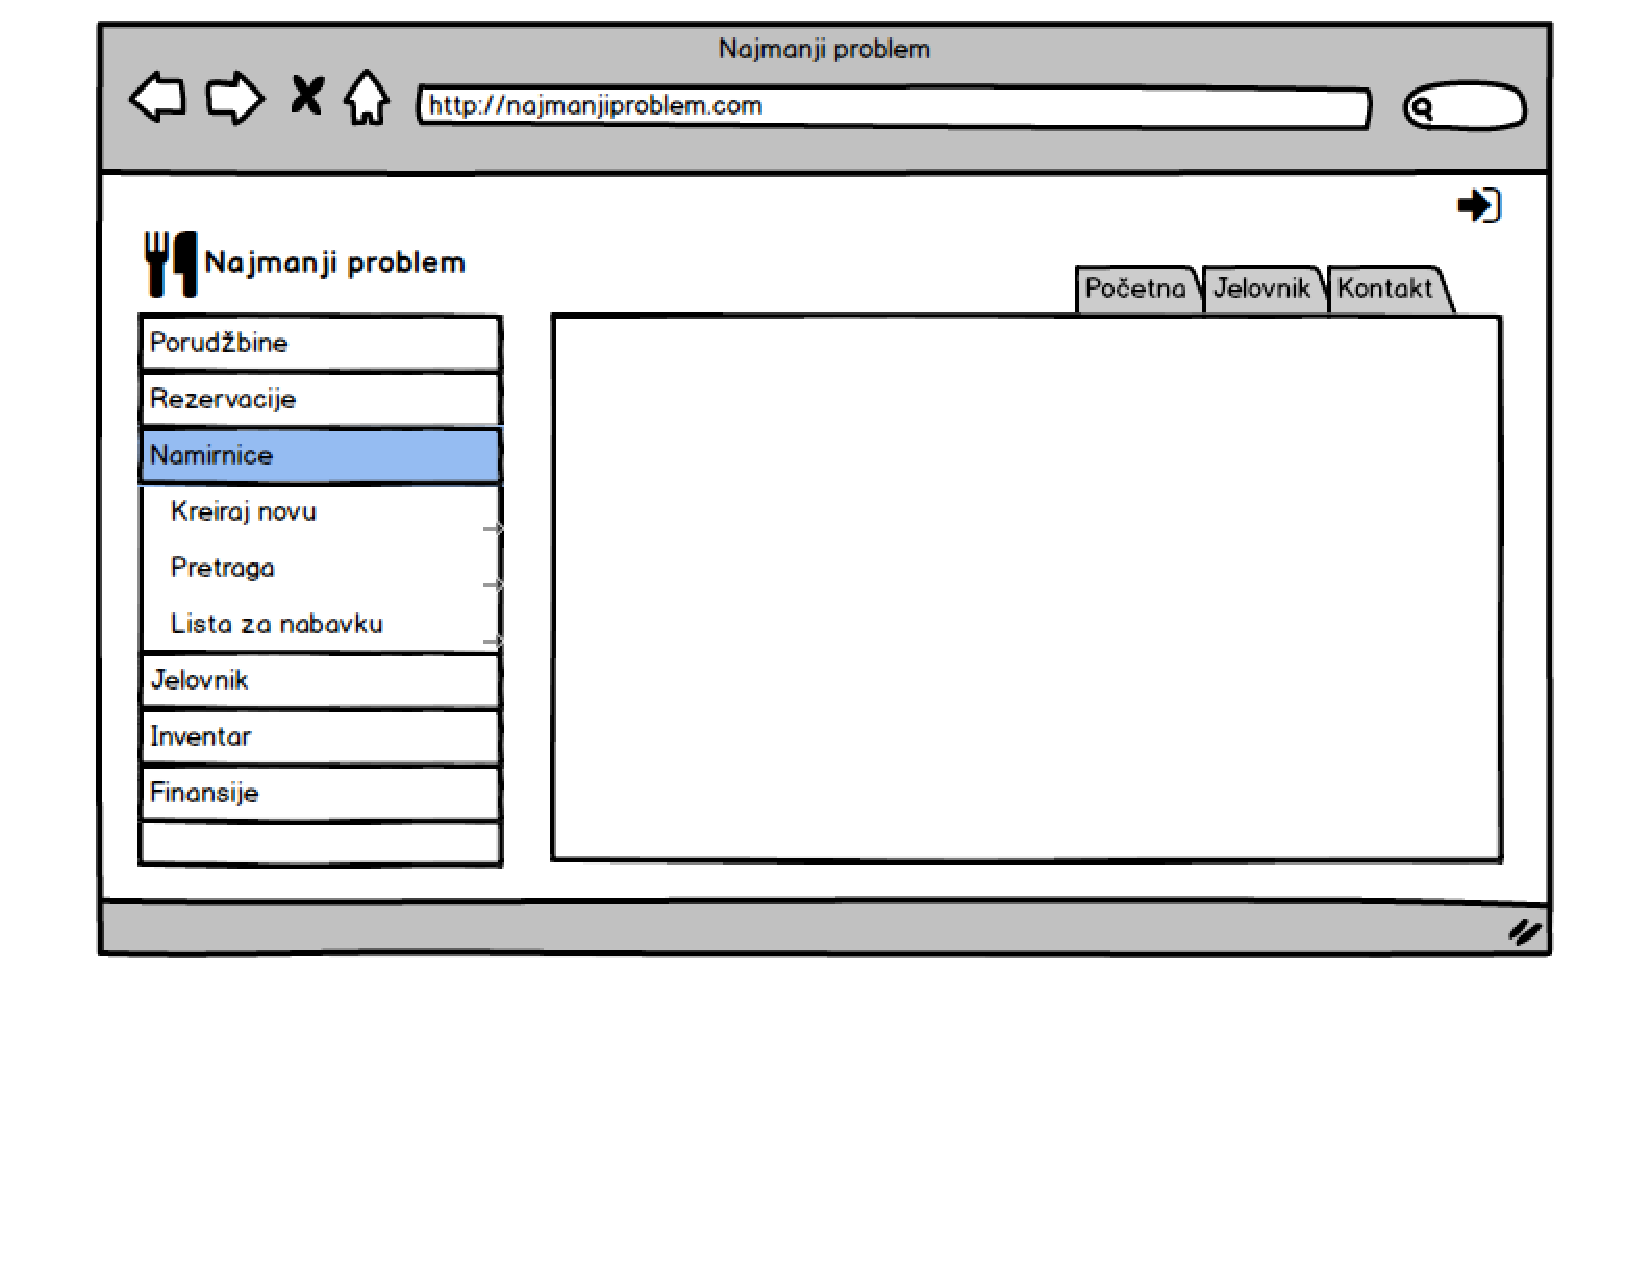
\includegraphics[
	page = 1,
    width=\textwidth,
    height=0.7\textheight,
    keepaspectratio]{1_PregledStanjaZalihaNamirnica.pdf}

\includegraphics[
	page = 2,
    width=\textwidth,
    height=0.7\textheight,
    keepaspectratio]{1_PregledStanjaZalihaNamirnica.pdf}

\includegraphics[
	page = 3,
    width=\textwidth,
    height=\textheight,
    keepaspectratio]{1_PregledStanjaZalihaNamirnica.pdf}

\includegraphics[
	page = 4,
    width=\textwidth,
    height=\textheight,
    keepaspectratio]{1_PregledStanjaZalihaNamirnica.pdf}

\includegraphics[
	page = 5,
    width=\textwidth,
    height=\textheight,
    keepaspectratio]{1_PregledStanjaZalihaNamirnica.pdf}
\vfill

\includegraphics[
	page = 6,
    width=\textwidth,
    height=\textheight,
    keepaspectratio]{1_PregledStanjaZalihaNamirnica.pdf}
\vfill

\includegraphics[
	page = 7,
    width=\textwidth,
    height=\textheight,
    keepaspectratio]{1_PregledStanjaZalihaNamirnica.pdf}
\vfill
\includegraphics[
	page = 8,
    width=\textwidth,
    height=\textheight,
    keepaspectratio]{1_PregledStanjaZalihaNamirnica.pdf}
\vfill

\subsubsection{Pregled inventara}
Na panelu \emph{Inventar} korisnik može da zahteva listu predmeta potrebnih za nabavku i odmah da ih i poruči. Korisnik može i da pretražuje postojeće predmete, kao i da kreira nove.\\\\

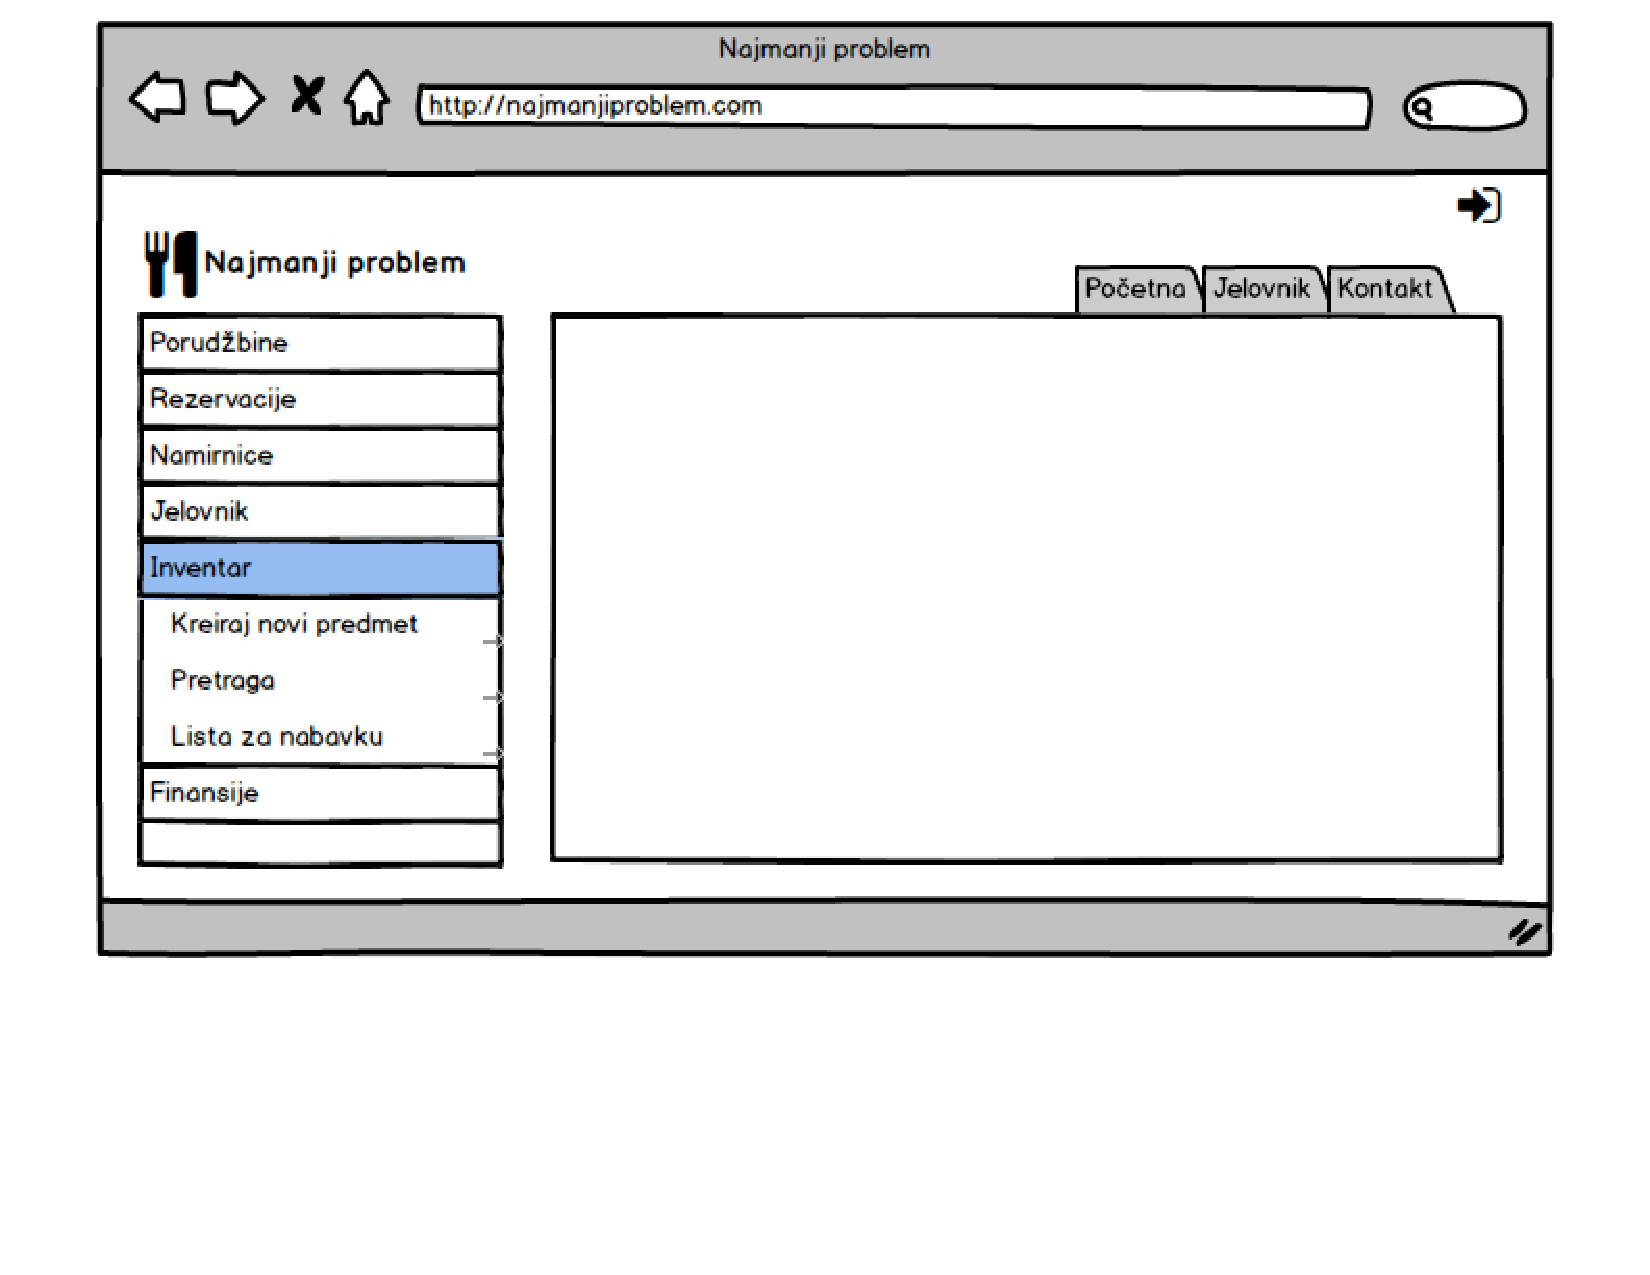
\includegraphics[
	page = 1,
    width=\textwidth,
    height=\textheight,
    keepaspectratio]{2_PregledInventara.pdf}

\includegraphics[
	page = 2,
    width=\textwidth,
    height=\textheight,
    keepaspectratio]{2_PregledInventara.pdf}

\includegraphics[
	page = 3,
    width=\textwidth,
    height=\textheight,
    keepaspectratio]{2_PregledInventara.pdf}

\includegraphics[
	page = 4,
    width=\textwidth,
    height=\textheight,
    keepaspectratio]{2_PregledInventara.pdf}

\includegraphics[
	page = 5,
    width=\textwidth,
    height=\textheight,
    keepaspectratio]{2_PregledInventara.pdf}

\includegraphics[
	page = 6,
    width=\textwidth,
    height=\textheight,
    keepaspectratio]{2_PregledInventara.pdf}

\newpage
\subsubsection{Pregled finansijskog stanja}
Na panelu \emph{Finansije} korisnik ima mogućnost pregleda postojećih izveštaja, kao i kreiranje novih.\\\\

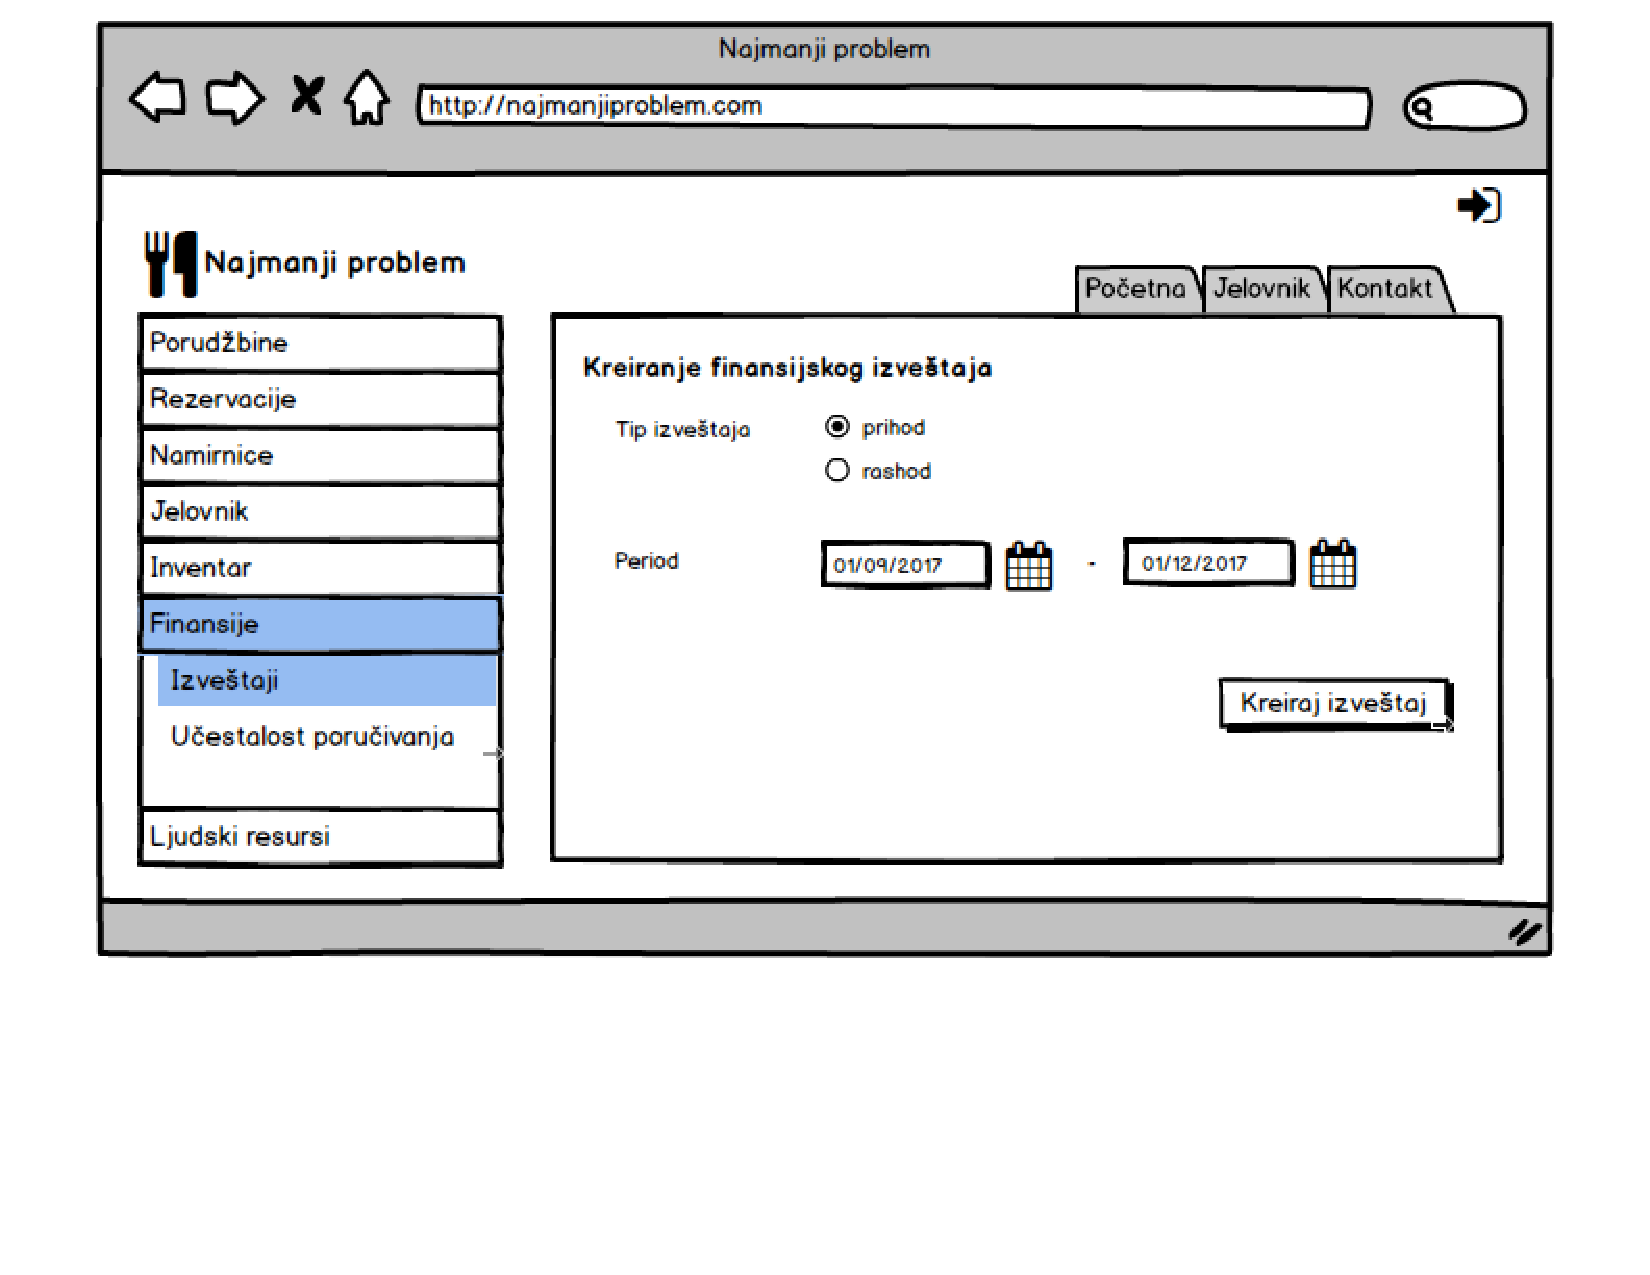
\includegraphics[
	page = 1,
    width=\textwidth,
    height=\textheight,
    keepaspectratio]{3_PregledFinansijskogStanja.pdf}

\includegraphics[
	page = 3,
    width=\textwidth,
    height=\textheight,
    keepaspectratio]{3_PregledFinansijskogStanja.pdf}
\includegraphics[
	page = 4,
    width=\textwidth,
    height=\textheight,
    keepaspectratio]{3_PregledFinansijskogStanja.pdf}

\includegraphics[
	page = 2,
    width=\textwidth,
    height=0.7\textheight,
    keepaspectratio]{3_PregledFinansijskogStanja.pdf}
 \newpage
\subsubsection{Upravljanje ljudskim resursima}
Na panelu \emph{Ljudski resursi} korisnik, u zavisnosti od dodeljenih prava, može da vidi/ izvrši određene akcije. U skladu sa tim akcije su : definisanje zahteva za odmor, kao i odgovor na iste.\\\\
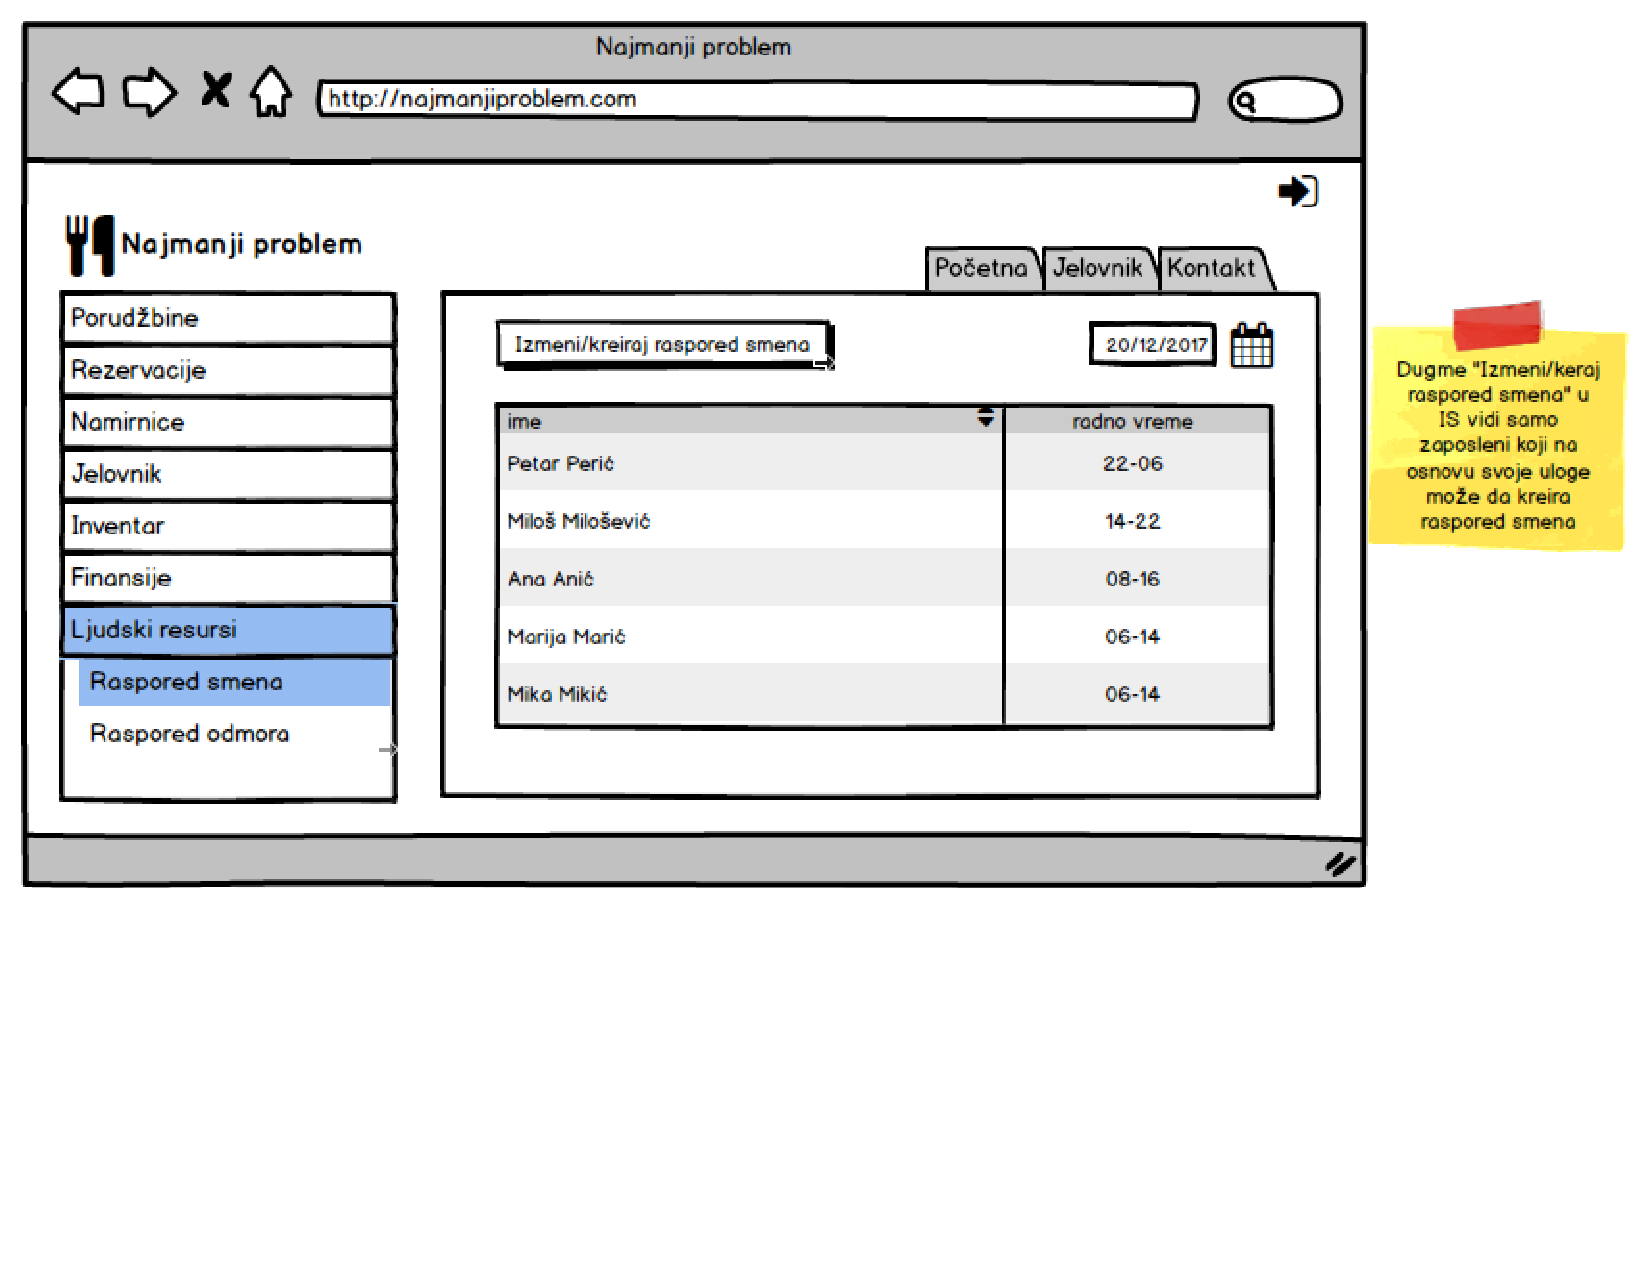
\includegraphics[
	page = 1,
    width=\textwidth,
    height=\textheight,
    keepaspectratio]{4_UpravljanjeLjudskimResursima.pdf}
 \vfill
\includegraphics[
	page = 2,
    width=\textwidth,
    height=\textheight,
    keepaspectratio]{4_UpravljanjeLjudskimResursima.pdf}
\noindent
\includegraphics[
	page = 3,
    width=\textwidth,
    height=\textheight,
    keepaspectratio]{4_UpravljanjeLjudskimResursima.pdf}
\includegraphics[
	page = 4,
    width=\textwidth,
    height=\textheight,
    keepaspectratio]{4_UpravljanjeLjudskimResursima.pdf}
\includegraphics[
	page = 5,
    width=\textwidth,
    height=\textheight,
    keepaspectratio]{4_UpravljanjeLjudskimResursima.pdf}
\includegraphics[
	page = 6,
    width=\textwidth,
    height=\textheight,
    keepaspectratio]{4_UpravljanjeLjudskimResursima.pdf}
\includegraphics[
	page = 7,
    width=\textwidth,
    height=\textheight,
    keepaspectratio]{4_UpravljanjeLjudskimResursima.pdf}
\subsubsection{Prihvatanje rezervacija gostiju}
Na panelu \emph{Rezervacije} korisnik može da prihvati zahteve za rezervaciju ili da obriše otkazane.\\\\
 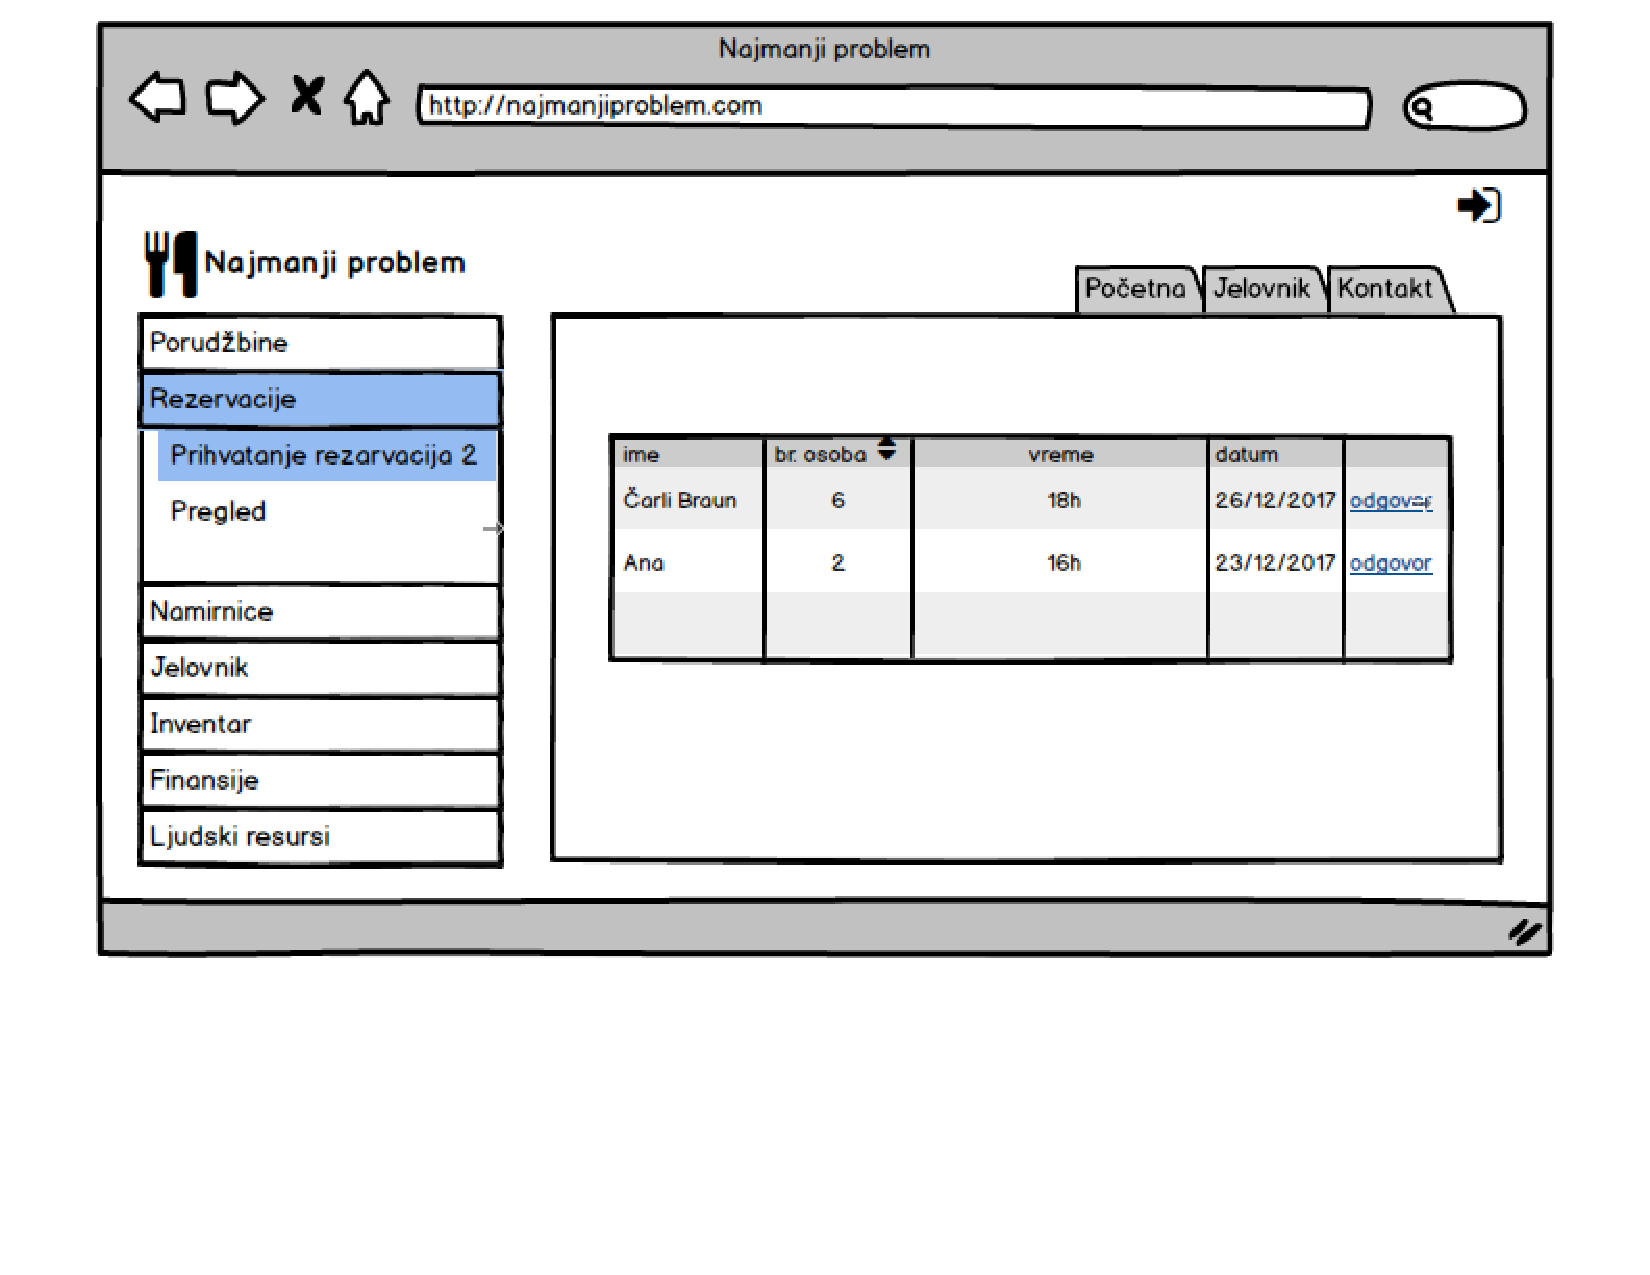
\includegraphics[
	page = 1,
    width=\textwidth,
    height=\textheight,
    keepaspectratio]{5_PrihvatanjeRezervacijaGostiju_Zaposleni.pdf}
\includegraphics[
	page = 2,
    width=\textwidth,
    height=0.5\textheight,
    keepaspectratio]{5_PrihvatanjeRezervacijaGostiju_Zaposleni.pdf}
\vfill
\includegraphics[
	page = 3,
    width=\textwidth,
    height=\textheight,
    keepaspectratio]{5_PrihvatanjeRezervacijaGostiju_Zaposleni.pdf}
    
\includegraphics[
	page = 4,
    width=\textwidth,
    height=\textheight,
    keepaspectratio]{5_PrihvatanjeRezervacijaGostiju_Zaposleni.pdf}
   

\subsubsection{Prihvatanje online porudžbina}
Na panelu \emph{Porudžbine}, korisnik može da : vidi novopristigle porudžbine, vidi spisak svih i izvrši odgovarajuće akcije sa njima (prihvatanje, označavanje za dostavu...).\\
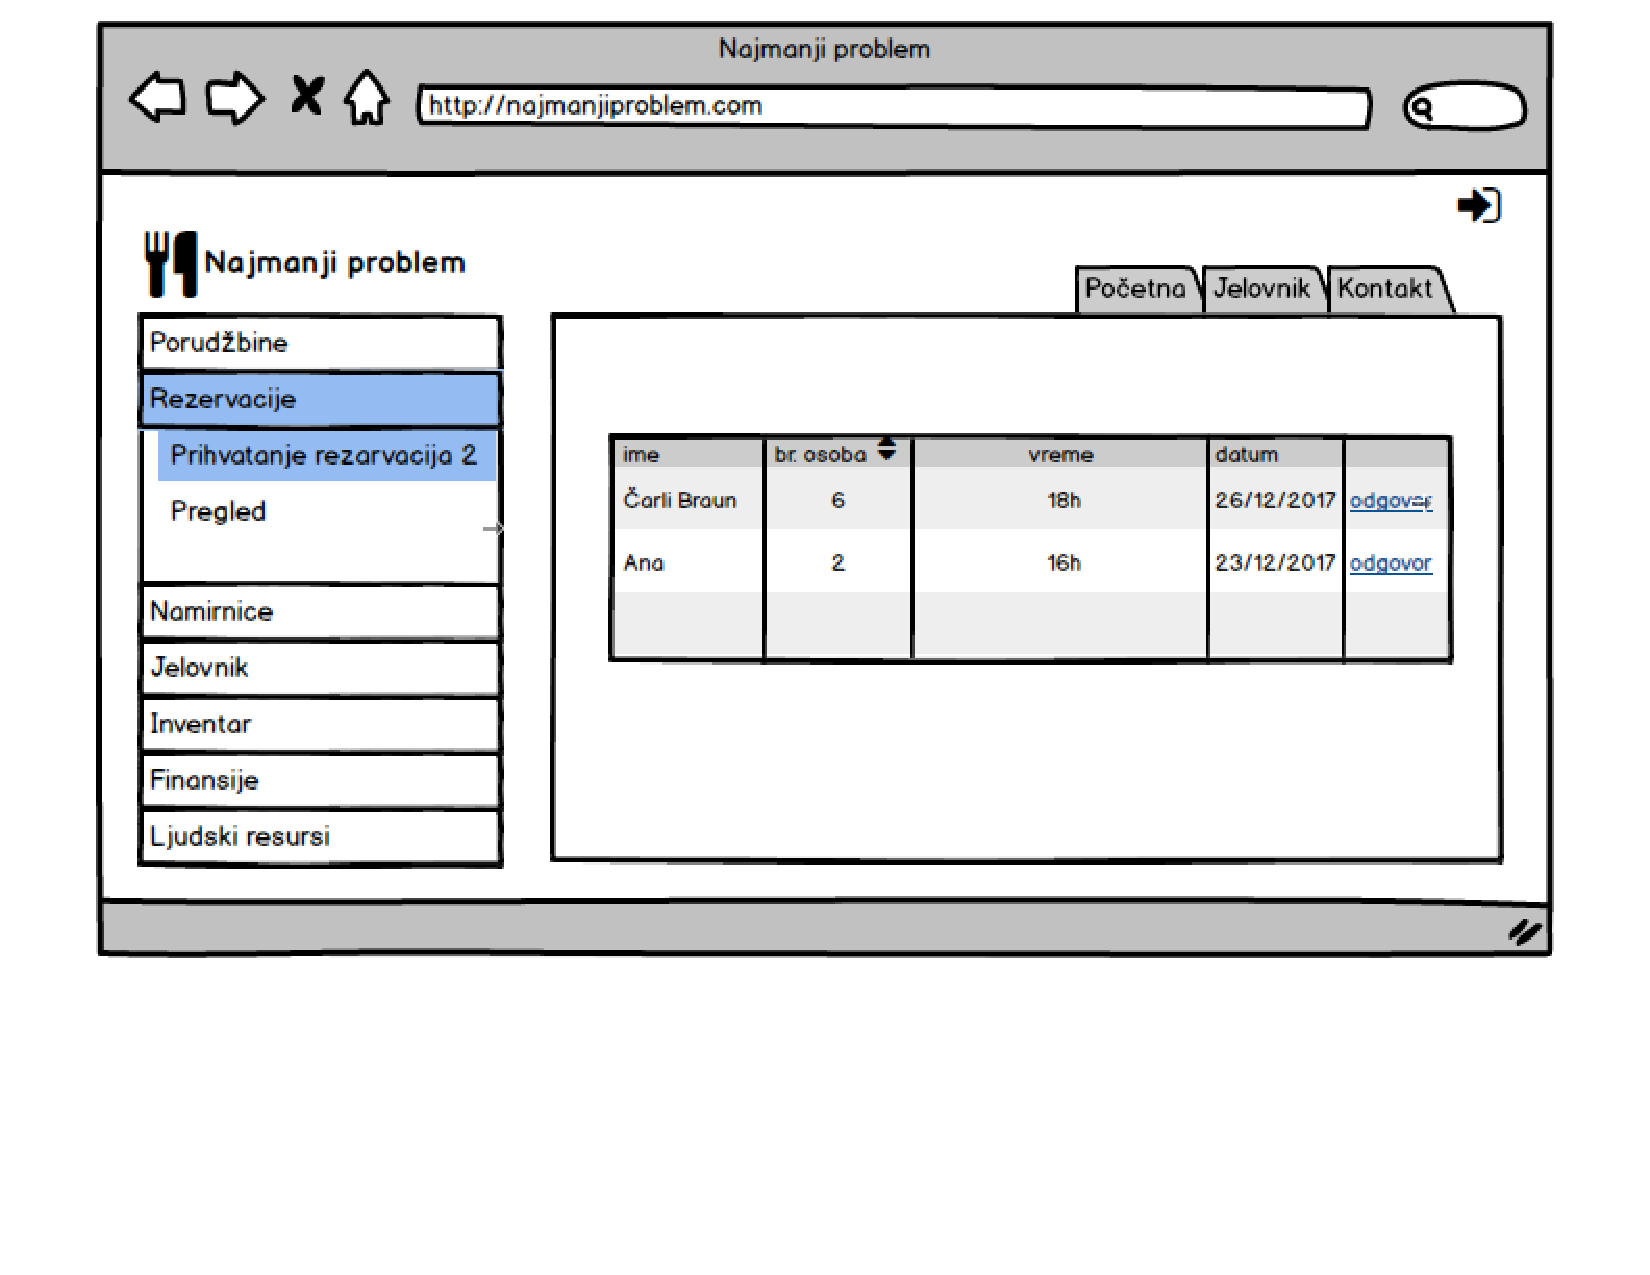
\includegraphics[
	page = 1,
    width=\textwidth,
    height=\textheight,
    keepaspectratio]
{5_PrihvatanjeRezervacijaGostiju_Zaposleni.pdf}
\vfill
\includegraphics[
	page = 2,
    width=\textwidth,
    height=\textheight,
    keepaspectratio]
{5_PrihvatanjeRezervacijaGostiju_Zaposleni.pdf}
\vfill
\includegraphics[
	page = 3,
    width=\textwidth,
    height=\textheight,
    keepaspectratio]
{5_PrihvatanjeRezervacijaGostiju_Zaposleni.pdf}
\includegraphics[
	page = 4,
    width=\textwidth,
    height=\textheight,
    keepaspectratio]
{5_PrihvatanjeRezervacijaGostiju_Zaposleni.pdf}

\subsection{Deo aplikacije namenjen za mušterije}

\subsubsection{Rezervacija stola}
Korisnik na panelu \emph{Rezervacije}, uz ostavljanje odgovarajućih podataka i informacija, može da izvrši rezervacije mesta.\\

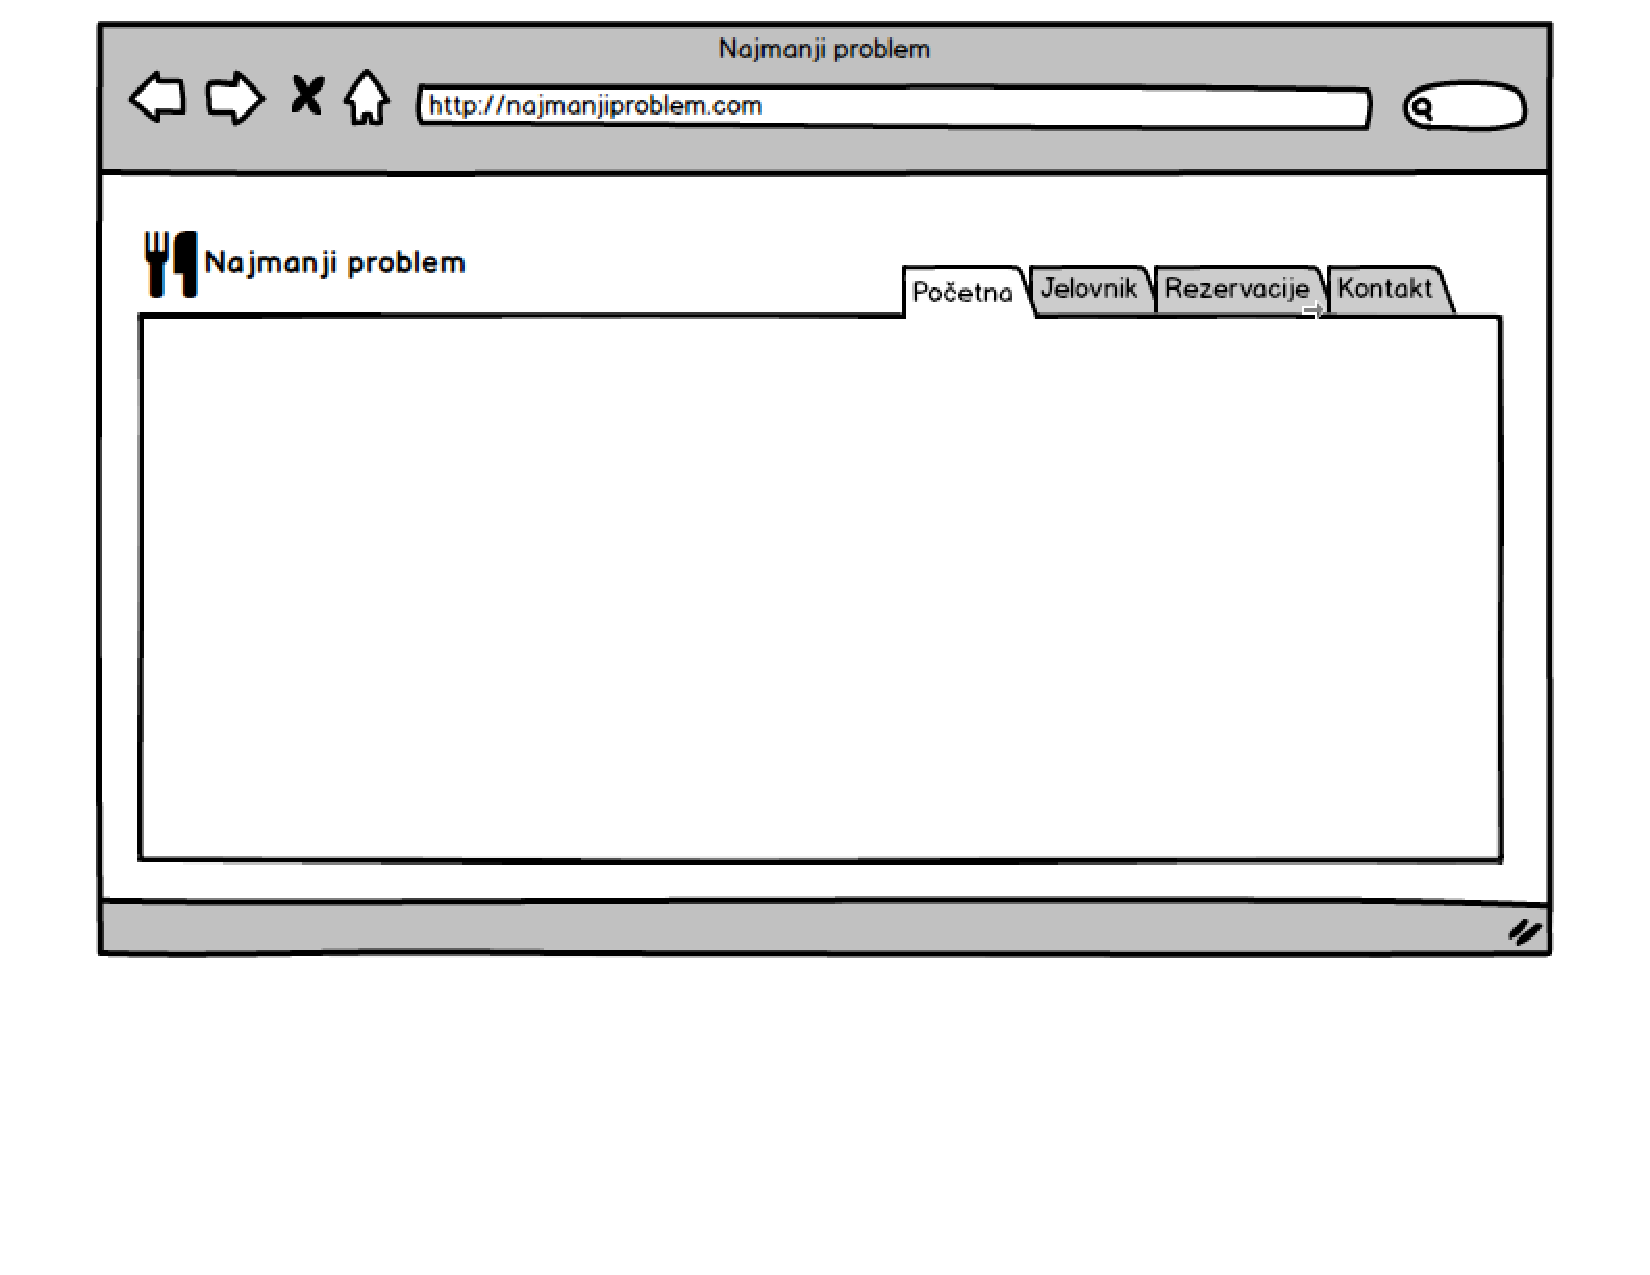
\includegraphics[
	page = 1,
    width=\textwidth,
    height=\textheight,
    keepaspectratio]{5_PrihvatanjeRezervacijaGostiju_Gost.pdf}
\vfill
\includegraphics[
	page = 2,
    width=\textwidth,
    height=\textheight,
    keepaspectratio]{5_PrihvatanjeRezervacijaGostiju_Gost.pdf}
\includegraphics[
	page = 3,
    width=\textwidth,
    height=\textheight,
    keepaspectratio]{5_PrihvatanjeRezervacijaGostiju_Gost.pdf}

\includegraphics[
	page = 4,
    width=\textwidth,
    height=\textheight,
    keepaspectratio]{5_PrihvatanjeRezervacijaGostiju_Gost.pdf}

\subsubsection{Online naručivanje}
Korisnik odabirom obroka, u panelu \emph{Jelovnik}, i ostavljanjem odgovarajućih kontakt informacija, može da izvrši narudžbinu.\\

\includegraphics[
	page = 1,
    width=\textwidth,
    height=\textheight,
    keepaspectratio]{6_OnlineNarucivanjeIDostava_Gost.pdf}

\includegraphics[
	page = 2,
    width=\textwidth,
    height=\textheight,
    keepaspectratio]{6_OnlineNarucivanjeIDostava_Gost.pdf}

\includegraphics[
	page = 3,
    width=\textwidth,
    height=\textheight,
    keepaspectratio]{6_OnlineNarucivanjeIDostava_Gost.pdf}
\pagebreak
\section{Arhitektura, alati i tehnologije}

Najmanji Problem je implementiran kao veb aplikacija. Aplikacija se sastoji od početne strane, sa mogućnošću prijavljivanja, kao i odvojene privilegije pristupa podacima od strane mušterije i zaposlenog. Zaposleni nakon autentifikacije dobija pristup stranicama koje se tiču jelovnika, inventara, namirnica i porudžbina. Mušterija može bez autentifikacije pristupiti aplikaciji, međutim za kreiranje rezervacije i porudžbine je neophodno da unese mejl adresu ili kontakt telefon.\\

\includegraphics[
page = 1,
width=\textwidth,
height=\textheight,
keepaspectratio]
{arhitektura.png}\\

Za izradu aplikacije korišćen je PHP razvojni okvir Laravel. Laravel je noviji MVC razvojni okvir za čije korišćenje je neophodan je Composer. Composer je alat za upravljanje zavisnim paketima u aplikacijama napisanim u PHP-u. Instalacija Composer-a podrazumeva preuzimanje datoteka određenog paketa i dodavanje istih samoj aplikaciji.\\

MVC deli sve što aplikacija sadrži na tri dela:
\begin{itemize}
	\item \textbf{Model} sadrži opis podataka i operacija nad njima. To je skup klasa koje opisuju sve entitete iz informacionog sistema. Primer modela su klase Order.php i OrderProduct.php. Prva opisuje porudžbine u aplikaciji, a druga elemente porudžbine.
	\item \textbf{View} ili pogled prikazuje podatke iz modela u formatu pogodnom za interakciju kao komponentu korisničkog interfejsa. Za svaki slučaj upotrebe kreiran je jedan view. U ovom delu su korišćeni HTML, CSS i JavaScript. Primer pogleda može biti stranica svih novih/neobrađenih online porudžbina.
	\item \textbf{Controller} obavlja komunikaciju između pogleda i modela, u zavisnosti od koirsnikovog unosa. Sadrži pripremu podataka za pogled, proračune, kao i njihovu pripremu pre slanja na obradu modelu. Primer kontrolera je OrderController.php koji sadrži metod za pripremu podataka koji su neophodni za prikazivanje stranice sa neobrađenih porudžbinama.
\end{itemize}

Za svaku klasu iz modela, kreirana je odgovarajuća tabela u bazi koju on opisuje. Sloj podataka je implementiran tako što je korišćen MySQL, verzija 5.7.19. Neke tabele su kreirane korišćenjem phpMyAdmin alata (verzija 4.7.4), međutim uglavnom su korišćene prednosti Laravela, pa su kreirane pomoću artisana. Artisan kreira PHP skripte (migraciju) za kreiranje i brisanje jedne tabele baze podataka za dati model. phpMyAdmin i MySQL su korišćeni u okviru softverskog paketa WAMP, verzija 3.1.0.\\

Laravel brine o konekciji na bazu, nisu potrebna dodatna podešavanja i ekstenzije, dovoljno je samo u konfiguracionom fajlu database.php upisati neophodne paramatre. \\

Pored navedenih tehnologija koje su korišćene u svrhu kreiranja veb aplikacije, za opis informaciong sistema korišćeni su i:
\begin{itemize}
	\item Visual Paradigm, verzija 14.2 - opis slučajeva upotrebe, dijagrami aktivnosti, dijagram baze podataka
	\item Balsamiq Mockups, verzija 3 - korisnički interfejs
\end{itemize}
\end{document}
